\documentclass[autodetect-engine, dvipdfmx-if-dvi, base=11pt, oneside, ja=standard]{bxjsreport}
% !TEX encoding = UTF-8 Unicode
\usepackage{graphicx}
\usepackage{text}
\usepackage{comment}

% 日本語フォント設定
\usepackage[sourcehan-jp, nfssonly, deluxe]{luatexja-preset}

% 強調(\emph)をボールドゴシックに設定
\let\emph\relax
\DeclareTextFontCommand{\emph}{\gtfamily\bfseries}

% チャプタータイトルの設定
\usepackage[Glenn]{fncychap}
\ChTitleVar{\bfseries\Large\mcfamily\rmfamily}
\makeatletter
\renewcommand{\DOCH}{%
  \settoheight{\myhi}{\CTV\FmTi{Test}}
  \setlength{\py}{\baselineskip}
  \addtolength{\py}{\RW}
  \addtolength{\py}{\myhi}
  \setlength{\pyy}{\py}
  \addtolength{\pyy}{-1\RW}
  \raggedright
  \CNV\FmN{\@chapapp}\space\CNoV\thechapter\CNV\FmN{\@chappos}
  \hskip 3pt\mghrulefill{\RW}\rule[-1\pyy]{2\RW}{\py}\par\nobreak
}
\makeatother

% GitのコミットIDを埋め込む用
\input{vc.tex}

%%% Cover

\title{Stuff Goes Bad:\protect\\ Erlang in Anger}
\author{Fred Hébert 著、elixir.jp 訳}

\date{%
  \today \\
  Git commit ID: \href{https://github.com/ymotongpoo/erlang-in-anger}{\GITAbrHash}
}

\begin{document}
\frontmatter

\maketitle

\includepdf[pagecommand={\thispagestyle{empty}}]{graphics/cover.pdf}

%%% Copyright page
\clearpage
\thispagestyle{fancy}

\fancyhf{} % remove everything
\renewcommand{\headrulewidth}{0pt} % remove lines as well
\renewcommand{\footrulewidth}{0pt}

\vspace*{\fill}


\begin{center}
\includegraphics[width=100pt]{by-nc-sa.eps}
\end{center}

\begin{center}
%\emph{Stuff Goes Bad: Erlang in Anger} by Fred Hébert and Heroku is licensed under a \href{http://creativecommons.org/licenses/by-nc-sa/4.0/}{Creative Commons Attribution-NonCommercial-ShareAlike 4.0 International License}.
Fred Hébert および Heroku社著の \emph{Stuff Goes Bad: Erlang in Anger} は \href{http://creativecommons.org/licenses/by-nc-sa/4.0/}{クリエイティブ・コモンズ 表示 - 非営利 - 継承 4.0 国際ライセンス} として公開されています。
\end{center}

%Thanks for the additional work, reviewing, and/or editing done by:
次の皆様のサポート、レビュー、そして編集に感謝します。

%\emph{Jacob Vorreuter}, \emph{Seth Falcon}, \emph{Raoul Duke}, \emph{Nathaniel Waisbrot}, \emph{David Holland}, \emph{Alisdair Sullivan}, \emph{Lukas Larsson}, \emph{Tim Chevalier}, \emph{Paul Bone}, \emph{Jonathan Roes}, \emph{Roberto Aloi}, \emph{Dmytro Lytovchenko}, and \emph{Tristan Sloughter}.
\emph{Jacob Vorreuter}、\emph{Seth Falcon}、\emph{Raoul Duke}、\emph{Nathaniel Waisbrot}、\emph{David Holland}、\emph{Alisdair Sullivan}、\emph{Lukas Larsson}、\emph{Tim Chevalier}、\emph{Paul Bone}、\emph{Jonathan Roes}、\emph{Roberto Aloi}、\emph{Dmytro Lytovchenko}、\emph{Tristan Sloughter}。

\null
\vfill
%\vspace*{\fill}
%The cover image is a modified version of \href{http://www.freeimages.com/photo/533163}{fallout shelter} by \href{http://www.freeimages.com/profile/drouu}{drouu} on \href{http://sxc.hu}{sxc.hu}.
表紙の画像は \href{http://sxc.hu}{sxc.hu} に掲載されている \href{http://www.freeimages.com/profile/drouu}{drouu} による \href{http://www.freeimages.com/photo/533163}{fallout shelter} を改変したものです。
\cfoot{\emph{v1.1.0}}
\rfoot{\emph{2016-04-06}}


%% License as of Monday, August 18, 2014:
%%
%% you may use any of my photos, original or modified, for any purpose whatsoever (personal, non-profit, or commercial; for web or print). you do not need to contact me prior to or after using one of my photos, though a comment or note is always appreciated if you have the opportunity.
%%
%% you may not claim ownership or copyright of my photos. seriously, i have an orbital karma gun and i'm not afraid to use it.


\clearpage
%%%

\tableofcontents

\listoffigures

%% Colors of figure refs for text
\hypersetup{linkcolor=violet}

%\chapter*{Introduction}
\chapter*{はじめに}
\markboth{\MakeUppercase{Introduction}}{}
%\addcontentsline{toc}{chapter}{Introduction}
\addcontentsline{toc}{chapter}{はじめに}
\label{chap:introduction}
\pagenumbering{arabic}
\setcounter{page}{1}


%\section*{On Running Software}
\section*{ソフトウェアを実行するにあたって}
%\addcontentsline{toc}{section}{On Running Software}
\label{sec:on-running-software}

%There's something rather unique in Erlang in how it approaches failure compared to most other programming languages. There's this common way of thinking where the language, programming environment, and methodology do everything possible to prevent errors. Something going wrong at run-time is something that needs to be prevented, and if it cannot be prevented, then it's out of scope for whatever solution people have been thinking about.

他のプログラミング言語と比較して、Erlangには障害が起きた場合の対処方法がかなり独特な部分があります。
他のプログラミング言語には、その言語自体や開発環境、開発手法といったものがエラーを防ぐためにできる限りのことをしてくれる、という共通の考え方があります。
実行時に何かがおかしくなるということは予防する必要があるもので、予防できなかった場合には、人々が考えてきたあらゆる解決策の範囲を超えてしまいます。

%The program is written once, and after that, it's off to production, whatever may happen there. If there are errors, new versions will need to be shipped.
プログラムは一度書かれると、本番環境に投入され、そこではあらゆることが発生するでしょう。
エラーがあったら、新しいバージョンを投入する必要がでてきます。

%Erlang, on the other hand, takes the approach that failures will happen no matter what, whether they're developer-, operator-, or hardware-related. It is rarely practical or even possible to get rid of all errors in a program or a system.\footnote{life-critical systems are usually excluded from this category} If you can deal with some errors rather than preventing them at all cost, then most undefined behaviours of a program can go in that "deal with it" approach.
一方で、Erlangでは障害というものは、それが開発者によるもの、運用者によるもの、あるいはハードウェアによるもの、それらのどれであろうとも起きるものである、という考え方に沿っています。
プログラムやシステム内のすべてのエラーを取り除くというのは非実用的かつ不可能に近いものです。\footnote{生命に関わるシステムは通常この議論の対象外です。}
エラーをあらゆるコストを払って予防するのではなく、エラーにうまく対処できれば、プログラムのたいていの予期せぬ動作もその「なんとかする」手法でうまく対応できるでしょう。

%This is where the "Let it Crash"\footnote{Erlang people now seem to favour "let it fail", given it makes people far less nervous.} idea comes from: Because you can now deal with failure, and because the cost of weeding out all of the complex bugs from a system before it hits production is often prohibitive, programmers should only deal with the errors they know how to handle, and leave the rest for another process (a supervisor) or the virtual machine to deal with.
これが「Let it Crash」\footnote{Erlang界隈の人々は、最近は不安がらせないようにということで「Let it Fail」のほうを好んで使うようです。}という考え方の元になっています。
この考えを元にすると障害にうまく対処出来ること、かつシステム内のすべての複雑なバグが本番環境で発生する前に取り除くコストが極めて高いことから、プログラマーは対応方法がわかっているエラーだけ対処すべきで、それ以外は他のプロセス(やスーパーバイザー)や仮想マシンに任せるべきです。

%Given that most bugs are transient\footnote{131 out of 132 bugs are transient bugs (they're non-deterministic and go away when you look at them, and trying again may solve the problem entirely), according to Jim Gray in \href{http://www.hpl.hp.com/techreports/tandem/TR-85.7.html}{Why Do Computers Stop and What Can Be Done About It?}}, simply restarting processes back to a state known to be stable when encountering an error can be a surprisingly good strategy.
たいていのバグが一時的なものであると仮定する\footnote{Jim Grayの\href{http://www.hpl.hp.com/techreports/tandem/TR-85.7.html}{Why Do Computers Stop and What Can Be Done About It?}によれば、132個中131このバグが一時的なもの(非決定的で調査するときにはなくなっていて、再実行することで問題が解決するもの)です。}と、エラーに遭遇したときに単純にプロセスを再起動して安定して動いていた状態に戻すというのは、驚くほど良い戦略になりえます。

%Erlang is a programming environment where the approach taken is equivalent to the human body's immune system, whereas most other languages only care about hygiene to make sure no germ enters the body. Both forms appear extremely important to me. Almost every environment offers varying degrees of hygiene. Nearly no other environment offers the immune system where errors at run time can be dealt with and seen as survivable.
Erlangというのは人体の免疫システムと同様の手法が取られているプログラミング環境です。一方で、他のたいていの言語は体内に病原菌が一切入らないようにするような衛生についてだけを考えています。どちらも私にとって極めて重要なプログラミング環境ものです。ほぼすべての環境でそれぞれに衛生状況が異なります。実行時のエラーがうまく対処されて、そのまま生き残れるような治癒の仕組みを持っているプログラミング環境はErlangの他にほとんどありません。

%Because the system doesn't collapse the first time something bad touches it, Erlang/OTP also allows you to be a doctor. You can go in the system, pry it open right there in production, carefully observe everything inside as it runs, and even try to fix it interactively. To continue with the analogy, Erlang allows you to perform extensive tests to diagnose the problem and various degrees of surgery (even very invasive surgery), without the patients needing to sit down or interrupt their daily activities.
Erlangではシステムになにか悪いことが起きてもすぐにはシステムが落ちないので、Erlang/OTPではあなたが医者のようにシステムを診察する術も提供してくれます。
システムの内部に入って、本番環境のその場でシステム内部を確認してまわって、実行中に内部をすべて注意深く観察して、ときには対話的に問題を直すことすらできるようになっています。
このアナロジーを使い続けると、Erlangは、患者に診察所に来てもらったり、患者の日々の生活を止めることなく、問題を検出するための広範囲に及ぶ検査を実行したり、様々な種類の手術(非常に侵襲性の高い手術でさえも)できるようにしてくれています。

%This book intends to be a little guide about how to be the Erlang medic in a time of war. It is first and foremost a collection of tips and tricks to help understand where failures come from, and a dictionary of different code snippets and practices that helped developers debug production systems that were built in Erlang.
本書は戦時においてErlang衛生兵になるためのちょっとしたガイドになるよう書かれました。本書は障害の発生原因を理解する上で役立つ秘訣や裏ワザを集めた初めての書籍であり、またErlangで作られた本番システムを開発者がデバッグするときに役立った様々なコードスニペットや実戦経験をあつめた辞書でもあります。

\section*{Who is this for?}
%\addcontentsline{toc}{section}{Who is this for?}
\label{sec:who-is-this-for}

This book is not for beginners. There is a gap left between most tutorials, books, training sessions, and actually being able to operate, diagnose, and debug running systems once they've made it to production. There's a fumbling phase implicit to a programmer's learning of a new language and environment where they just have to figure how to get out of the guidelines and step into the real world, with the community that goes with it.

This book assumes that the reader is proficient in basic Erlang and the OTP framework. Erlang/OTP features are explained as I see fit — usually when I consider them tricky — and it is expected that a reader who feels confused by usual Erlang/OTP material will have an idea of where to look for explanations if necessary\footnote{I do recommend visiting \href{http://learnyousomeerlang.com}{Learn You Some Erlang} or the regular \href{http://www.erlang.org/erldoc}{Erlang Documentation} if a free resource is required}.

What is not necessarily assumed is that the reader knows how to debug Erlang software, dive into an existing code base, diagnose issues, or has an idea of the best practices about deploying Erlang in a production environment\footnote{Running Erlang in a screen or tmux session is \emph{not} a deployment strategy.}.

\section*{How To Read This Book}
%\addcontentsline{toc}{section}{How To Read This Book}
\label{sec:how-to-read-this-book}

This book is divided in two parts. 

Part \ref{part:writing-applications} focuses on how to write applications. It includes how to dive into a code base (Chapter \ref{chap:how-to-dive-into-a-code-base}), general tips on writing open source Erlang software (Chapter \ref{chap:building-open-source-erlang-software}), and how to plan for overload in your system design (Chapter \ref{chap:overload}).

Part \ref{part:diagnosing-applictions} focuses on being an Erlang medic and concerns existing, living systems. It contains instructions on how to connect to a running node (Chapter \ref{chap:connecting}), and the basic runtime metrics available (Chapter \ref{chap:runtime-metrics}). It also explains how to perform a system autopsy using a crash dump (Chapter \ref{chap:crash-dumps}), how to identify and fix memory leaks (Chapter \ref{chap:memory-leaks}), and how to find runaway CPU usage (Chapter \ref{chap:cpu-hogs}). The final chapter contains instructions on how to trace Erlang function calls in production using \otpapp{recon}\footnote{\href{http://ferd.github.io/recon/}{http://ferd.github.io/recon/} — a library used to make the text lighter, and with generally production-safe functions.} to understand issues before they bring the system down (Chapter \ref{chap:tracing}).

Each chapter is followed up by a few optional exercises in the form of questions or hands-on things to try if you feel like making sure you understood everything, or if you want to push things further.



\mainmatter

\part{Writing Applications}
\label{part:writing-applications}

%\chapter{How to Dive into a Code Base}
\chapter{コードベースへの飛び込み方}
\label{chap:how-to-dive-into-a-code-base}

%"Read the source" is one of the most annoying things to be told, but dealing with Erlang programmers, you'll have to do it often. Either the documentation for a library will be incomplete, outdated, or just not there. In other cases, Erlang programmers are a bit similar to Lispers in that they will tend to write libraries that will solve their problems and not really test or try them in other circumstances, leaving it to you to extend or fix issues that arise in new contexts.
「ソースを読め」というフレーズは言われるともっとも煩わしい言葉ではありますが、Erlangプログラマとしてやっていくのであれば、しばしばそうしなければならないでしょう。
ライブラリのドキュメントが不完全だったり、古かったり、あるいは単純にドキュメントが存在しなかったりします。
また他の理由として、ErlangプログラマはLisperに近しいところが少しあって、ライブラリを書くときには自身に起こっている問題を解決するために書いて、テストをしたり、他の状況で試したりということはあまりしない傾向にあります。そしてそういった別のコンテキストで発生する問題を直したり、拡張する場合は自分で行う必要があります。

%It's thus pretty much guaranteed you'll have to go dive in some code base you know nothing about, either because you inherited it at work, or because you need to fix it or understand it to be able to move forward with your own system. This is in fact true of most languages whenever the project you work on is not one you designed yourself.
したがって、仕事で引き継ぎがあった場合でも、自分のシステムと連携するために問題を修正したりあるいは中身を理解する場合でも、何も知らないコードベースに飛び込まなければならなくなることはまず間違いないでしょう。
これは取り組んでいるプロジェクトが自分自身で設計したわけではない場合はいつでも、たいていの言語でも同様です。

%There are three main types of Erlang code bases you'll encounter in the wild: raw Erlang code bases, OTP applications, and OTP releases. In this chapter, we'll look at each of these and try to provide helpful tips on navigating them.
世間にあるErlangのコードベースには主に3つの種類があります。1つめは生のErlangコードベース、2つめはOTPアプリケーション、3つめはOTPリリースです。
この章ではこれら3つのそれぞれに見ていき、それぞれを読み込んでいくのに役立つ秘訣をお教えします。

%\section{Raw Erlang}
\section{生のErlang}
\label{sec:dive-raw-erlang}

%If you encounter a raw Erlang code base, you're pretty much on your own. These rarely follow any specific standard, and you have to dive in the old way to figure out whatever happens in there.
生のErlangコードベースに遭遇したら、各自でなんとかしてください。こうしたコードはなにか特に標準に従っているわけでもないので、何が起きているかは自分で深い道に分け入っていかなければなりません。

%This means hoping for a \filename{README.md} file or something similar that can point to an entry point in the application, and going from there, or hoping for some contact information that can be used to ask questions to the author(s) of the library.
つまり、\filename{README.md}ファイルの類がアプリケーションのエントリーポイントを示してくれていて、さらにいえば、ライブラリ作者に質問するための連絡先情報などがあることを願うのみということです。

Fortunately, you should rarely encounter raw Erlang in the wild, and they are often beginner projects, or awesome projects that were once built by Erlang beginners and now need a serious rewrite. In general, the advent of tools such as \app{rebar3} and its earlier incarnations\footnote{\href{https://www.rebar3.org}{https://www.rebar3.org} — a build tool briefly introduced in Chapter \ref{chap:building-open-source-erlang-software}} made it so most people use OTP Applications.

%\section{OTP Applications}
\section{OTPアプリケーション}
\label{sec:dive-otp-applications}

%Figuring out OTP applications is usually rather simple. They usually all share a directory structure that looks like:
OTPアプリケーションを理解するのは通常かなり単純です。OTPアプリケーションはみな次のようなディレクトリ構造をしています。

\begin{VerbatimRaw}
doc/
ebin/
src/
test/
LICENSE.txt
README.md
rebar.config
\end{VerbatimRaw}

%There might be slight differences, but the general structure will be the same.
わずかな違いはあるかもしれませんが、一般的な構造は同じです。

%Each OTP application should contain an \emph{app file}, either \filename{ebin/<AppName>.app} or more often, \filename{src/<AppName>.app.src}\footnote{A build system generates the final file that goes in \filename{ebin}. Note that in these cases, many  \filename{src/<AppName>.app.src} files do not specify modules and let the build system take care of it.}. There are two main varieties of app files:
各OTPアプリケーションは \emph{appファイル} を持っていて、\filename{ebin/<AppName>.app}か、あるいはしばしば \filename{src/<AppName>.app.src} という名前になっているはずです。\footnote{ビルドシステムが最終的に \filename{ebin} にファイルを生成します。この場合、多くの \filename{src/<AppName>.app.src} ファイルはモジュールを示すものではなく、ビルドシステムがモジュール化の面倒を見ることになります。}
appファイルには主に2つの種類があります。

\includecode[erlang]{useragent.app.src}

%And:
そして

\includecode[erlang]{dispcount.app}

の2種類です。

%This first case is called a \emph{library application}, while the second case is a regular \emph{application}.
最初のケースは \emph{ライブラリアプリケーション} と呼ばれていて、2つめのケースは標準 \emph{アプリケーション} と呼ばれています。

%\subsection{Library Applications}
\subsection{ライブラリアプリケーション}
\label{subsec:dive-library-applications}

%Library applications will usually have modules named \module{\emph{appname}\_something}, and one module named \module{\emph{appname}}. This will usually be the interface module that's central to the library and contains a quick way into most of the functionality provided.
ライブラリアプリケーションは通常 \module{\emph{appname}\_something} というような名前のモジュールと、 \module{\emph{appname}} という名前のモジュールを持っています。
これは通常ライブラリの中心となるインターフェースモジュールで、提供される大半の機能がそこに含まれています。

%By looking at the source of the module, you can figure out how it works with little effort: If the module adheres to any given behaviour (\module{gen\_server}, \module{gen\_fsm}, etc.), you're most likely expected to start a process under one of your own supervisors and call it that way. If no behaviour is included, then you probably have a functional, stateless library on your hands. For this case, the module's exported functions should give you a quick way to understand its purpose.

モジュールのソースを見ることで、少しの労力でモジュールがどのように動作するか理解できます。もしモジュールが特定のビヘイビア(\module{gen\_server}や\module{gen\_fsm}など)を何度も使っているようであれば、おそらくスーパーバイザーの下でプロセスを起動して、然るべき方法で呼び出すことが想定されているでしょう。
ビヘイビアが一つもなければ、そこにあるのは関数のステートレスなライブラリです。この場合、モジュールのエクスポートされた関数を見ることで、このライブラリの目的を素早く理解できるでしょう。

\subsection{Regular Applications}
\label{subsec:dive-regular-applications}

For a regular OTP application, there are two potential modules that act as the entry point:

\begin{enumerate*}
	\item \module{\emph{appname}}
	\item \module{\emph{appname}\_app}
\end{enumerate*}

The first file should be similar in use to what we had in a library application (an entry point), while the second one will implement the \module{application} behaviour, and will represent the top of the application's process hierarchy. In some cases the first file will play both roles at once.

If you plan on simply adding the application as a dependency to your own app, then look inside \module{\emph{appname}} for details and information. If you need to maintain and/or fix the application, go for \module{\emph{appname}\_app} instead.

The application will start a top-level supervisor and return its \emph{pid}. This top-level supervisor will then contain the specifications of all the child processes it will start on its own\footnote{In some cases, the supervisor specifies no children: they will either be started dynamically by some function of the API or in a start phase of the application, or the supervisor is only there to allow OTP environment variables (in the \expression{env} tuple of the app file) to be loaded.}.

The higher a process resides in the tree, the more likely it is to be vital to the survival of the application. You can also estimate how important a process is by the order it is started (all children in the supervision tree are started in order, depth-first). If a process is started later in the supervision tree, it probably depends on processes that were started earlier.

Moreover, worker processes that depend on each other within the same application (say, a process that buffers socket communications and relays them to a finite-state machine in charge of understanding the protocol) are likely to be regrouped under the same supervisor and to fail together when something goes wrong. This is a deliberate choice, as it is usually simpler to start from a blank slate, restarting both processes, rather than trying to figure out how to recuperate when one or the other loses or corrupts its state.

The supervisor restart strategy reflects the relationship between processes under a supervisor:

\begin{itemize*}
	\item \expression{one\_for\_one} and \expression{simple\_one\_for\_one} are used for processes that are not dependent upon each other directly, although their failures will collectively be counted towards total application shutdown\footnote{Some developers will use \expression{one\_for\_one} supervisors when \expression{rest\_for\_one} is more appropriate. They require strict ordering to boot correctly, but forget about said order when restarting or if a predecessor dies.}.
	\item \expression{rest\_for\_one} will be used to represent processes that depend on each other in a linear manner.
	\item \expression{one\_for\_all} is used for processes that entirely depend on each other.
\end{itemize*}

This structure means it is easiest to navigate OTP applications in a top-down manner by exploring supervision subtrees. 

For each worker process supervised, the behaviour it implements will give a good clue about its purpose:

\begin{itemize*}
	\item a \module{gen\_server} holds resources and tends to follow client/server patterns (or more generally, request/response patterns)
	\item a \module{gen\_fsm} will deal with a sequence of events or inputs and react depending on them, as a Finite State Machine. It will often be used to implement protocols.
	\item a \module{gen\_event} will act as an event hub for callbacks, or as a way to deal with notifications of some sort.
\end{itemize*}

All of these modules will contain the same kind of structure: exported functions that represent the user-facing interface, exported functions for the callback module, and private functions, usually in that order.

Based on their supervision relationship and the typical role of each behaviour, looking at the interface to be used by other modules and the behaviours implemented should reveal a lot of information about the program you're diving into.

\subsection{Dependencies}
\label{subsec:dive-dependencies}

All applications have dependencies\footnote{At the very least on the \module{kernel} and \module{stdlib} applications}, and these dependencies will have their own dependencies. OTP applications usually share no state between them, so it's possible to know what bits of code depend on what other bits of code by looking at the app file only, assuming the developer wrote them in a mostly correct manner. Figure~\ref{fig:app-deps} shows a diagram that can be generated from looking at app files to help understand the structure of OTP applications.


\begin{figure}
  \includegraphics{app-deps-riak-cs.pdf}%
  \caption{Dependency graph of riak\_cs, Basho's open source cloud library.
  The graph ignores dependencies on common applications like kernel and stdlib. Ovals are applications, rectangles are library applications.}%
   \label{fig:app-deps}
\end{figure}

Using such a hierarchy and looking at each application's short description might be helpful to draw a rough, general map of where everything is located. To generate a similar diagram, find \app{recon}'s script directory and call \command{escript script/app\_deps.erl}\footnote{This script depends on graphviz}. Similar hierarchies can be found using the \module{observer}\footnote{\href{http://www.erlang.org/doc/apps/observer/observer\_ug.html}{http://www.erlang.org/doc/apps/observer/observer\_ug.html}} application, but for individual supervision trees. Put together, you may get an easy way to find out what does what in the code base.

\FloatBarrier

\section{OTP Releases}
\label{sec:dive-otp-releases}

OTP releases are not a lot harder to understand than most OTP applications you'll encounter in the wild. A release is a set of OTP applications packaged in a production-ready manner so it boots and shuts down without needing to manually call \function{application:start/2} for any app. Compiled releases may contain their own copy of the Erlang virtual machine with more or less libraries than the default distribution, and can be ready to run standalone. Of course there's a bit more to releases than that, but generally, the same discovery process used for individual OTP applications will be applicable here.

You'll usually have a file named \filename{relx.config} or a \term{relx} tuple in a \filename{rebar.config} file, which will state which top-level applications are part of the release and some options regarding their packaging. Relx-based releases can be understood by reading the project's wiki\footnote{\href{https://github.com/erlware/relx/wiki}{https://github.com/erlware/relx/wiki}}, or their documentation on the documentation sites of \app{rebar3}\footnote{\href{https://www.rebar3.org/docs/releases}{https://www.rebar3.org/docs/releases}} or \filename{erlang.mk}\footnote{\href{http://erlang.mk/guide/relx.html}{http://erlang.mk/guide/relx.html}}.

Other systems may depend on the configuration files used by \module{systools} or \module{reltool}, which will state all applications part of the release and a few\footnote{A lot} options regarding their packaging. To understand them, I recommend \href{http://learnyousomeerlang.com/release-is-the-word}{reading existing documentation on them}.

\section{Exercises}

\subsection*{Review Questions}

\begin{enumerate}
	\item How do you know if a code base is an application? A release?
	\item What differentiates an application from a library application?
	\item What can be said of processes under a \term{one\_for\_all} scheme for supervision?
	\item Why would someone use a \module{gen\_fsm} behaviour over a \module{gen\_server}?
\end{enumerate}

\subsection*{Hands-On}

Download the code at \href{https://github.com/ferd/recon\_demo}{https://github.com/ferd/recon\_demo}. This will be used as a test bed for exercises throughout the book. Given you are not familiar with the code base yet, let's see if you can use the tips and tricks mentioned in this chapter to get an understanding of it.

\begin{enumerate}
	\item Is this application meant to be used as a library? A standalone system?
	\item What does it do?
	\item Does it have any dependencies? What are they?
	\item The app's \filename{README} mentions being non-deterministic. Can you prove if this is true? How?
	\item Can you express the dependency chain of applications in there? Generate a diagram of them?
	\item Can you add more processes to the main application than those described in the \filename{README}? 
\end{enumerate}


%\chapter{Building Open Source Erlang Software}
\chapter{オープンソースのErlang製ソフトウェアをビルドする}
\label{chap:building-open-source-erlang-software}

%Most Erlang books tend to explain how to build Erlang/OTP applications, but few of them go very much in depth about how to integrate with the Erlang community doing Open Source work. Some of them even avoid the topic on purpose. This chapter dedicates itself to doing a quick tour of the state of affairs in Erlang.
多くのErlangに関する書籍はErlang/OTPアプリケーションのビルド方法に関しては説明していますが、Erlangのコミュニティが開発しているオープンソースとの連携方法まで含めた深い解説を行っているものはほとんどありません。
中には意図的にその話題を避けているものさえあります。本章ではErlangでのオープンソースとの連携に関して簡単に案内します。

%OTP applications are the vast majority of the open source code people will encounter. In fact, many people who would need to build an OTP release would do so as one umbrella OTP application.
世間で見かけるオープンソースコードの大半がOTPアプリケーションです。事実、OTPリリースをビルドする多くの人はひとかたまりのOTPアプリケーションとしてビルドしています。

%If what you're writing is a stand-alone piece of code that could be used by someone building a product, it's likely an OTP application. If what you're building is a product that stands on its own and should be deployed by users as-is (or with a little configuration), what you should be building is an OTP release.\footnote{The details of how to build an OTP application or release is left up to the Erlang introduction book you have at hand.}
あなたが書いているものがプロジェクトを作っている誰かに使われる可能性がある独立したコードであれば、おそらくそれはOTPアプリケーションでしょう。
あなたが作っているものがユーザーがそのままの形でデプロイするような単独で動作するプロダクトであれば、それはOTPリリースでしょう。\footnote{OTPアプリケーションとOTPリリースのビルドの仕方についてはお手元にあるErlangの入門書に譲ります。}

%The main build tools supported are \app{rebar3} and \app{erlang.mk}. The former is a build tool and package manager trying to make it easy to develop and release Erlang libraries and systems in a repeatable manner, while the latter is a very fancy makefile that offers a bit less for production and releases but allows more flexibility. In this chapter, I'll mostly focus on using \app{rebar3} to build things, given it's the de-facto standard, is a tool I know well, and that \app{erlang.mk} applications tend to also be supported by \app{rebar3} as dependencies (the opposite is also true).
サポートされている主なビルドツールは\app{rebar3}と\app{erlang.mk}です。前者はビルドツールでありパッケージマネージャーで、ErlangライブラリとErlang製システムを繰り返し使える形で簡単に開発してリリースできるようにしてくれるものです。一方で後者は特殊なmakefileで本番用やリリースにはそれほど向いていませんが、より柔軟な記述が出来るようになっています。
本章では、\app{rebar3}がデファクトスタンダードになっていること、自分がよく知っていること、また\app{erlang.mk}は\app{rebar3}の依存先としてサポートされている事が多いといった理由から、\app{rebar3}を使ったビルドに焦点をあてます。

%\section{Project Structure}
\section{プロジェクト構造}
\label{sec:project-structure}

%The structures of OTP applications and of OTP releases are different. An OTP application can be expected to have one top-level supervisor (if any) and possibly a bunch of dependencies that sit below it. An OTP release will usually be composed of multiple OTP applications, which may or may not depend on each other. This will lead to two major ways to lay out applications.
OTPアプリケーションとOTPリリースのプロジェクト構造は異なります。OTPアプリケーションは(あるとすれば)トップレベルスーパーバイザーを1つ持っていると想定できます。そしておそらく依存しているものがその下に固まってぶら下がっていると想定できます。
OTPリリースは通常複数のOTPアプリケーションから成り、それらがお互いに依存していることもあればそうでないこともあります。
これらの事実からアプリケーションの構成をする際に主に2つの方法に落ち着きます。

%\subsection{OTP Applications}
\subsection{OTPアプリケーション}
\label{subsec:building-otp-applications}

%For OTP applications, the proper structure is pretty much the same as what was explained in \ref{sec:dive-otp-applications}:
OTPアプリケーションでは、適切な構造は\ref{sec:dive-otp-applications}の節で説明したとおりです。

\begin{VerbatimText}
_build/
doc/
src/
test/
LICENSE.txt
README.md
rebar.config
rebar.lock
\end{VerbatimText}

%What's new in this one is the \filename{\_build/} directory and the \filename{rebar.lock} file, which will be generated automatically by \app{rebar3}\footnote{Some people package \app{rebar3} directly in their application. This was initially done to help people who had never used rebar3 or its predecessors use libraries and projects in a boostrapped manner. Feel free to install rebar3 globally on your system, or keep a local copy if you require a specific version to build your system.}.
ここで新しいのは\filename{\_build/}ディレクトリと\filename{rebar.lock}ファイルです。
これらは\app{rebar3}によって自動的に生成されます。\footnote{人によっては\app{rebar3}をアプリケーション内に直接パッケージします。これはrebar3やその前身を使ったことがない人がライブラリやプロジェクトとブートストラップできるようになされていたものです。自分のシステムのグローバルにrebar3をインストールして問題ありません。自分のシステムをビルドするのに特定のバージョンが必要であればローカルにコピーを持っておいても良いでしょう。}

%This is the directory where \app{rebar3} places all build artifacts for a project, including local copies of libraries and packages required for it to work. No mainstream Erlang tool installs packages globally\footnote{Except as a local cache of unbuilt packages.}, preferring to instead keep everything project-local to avoid inter-project conflicts.
このディレクトリに\app{rebar3}がプロジェクトのすべてのビルドアーティファクトを置きます。動作させるのに必要なライブラリやパッケージのローカルコピーなどもそこに含まれます。
主要なErlangツールはパッケージをグローバルにはインストールせず、\footnote{まだビルドされていないパッケージのローカルキャッシュは除きます。}かわりにプロジェクト間での衝突を避けるためにすべてをプロジェクトローカルに保存します。

%Such dependencies can be specified for \app{rebar3} by adding a few config lines to \filename{rebar.config}:
このような依存関係は\filename{rebar.config}に数行設定を追加するだけで\app{rebar3}に指定できます。

\begin{VerbatimText}
{deps, [
  %% Hex.pm Packages
  myapp,
  {myapp,"1.0.0"},
  %% source dependencies 
  {myapp, {git, "git://github.com/user/myapp.git", {ref, "aef728"}}},
  {myapp, {git, "https://github.com/user/myapp.git", {branch, "master"}}},
  {myapp, {hg, "https://othersite.com/user/myapp", {tag, "3.0.0"}}}
 ]}.
\end{VerbatimText}

%Dependencies are fetched directly from a \app{git} (or \app{hg}) source or as a package from \href{https://hex.pm}{\app{hex.pm}} in a level-order traversal. They can then be compiled, and specific compile options can be added with the \expression{\{erl\_opts, List\}.} option in the config file\footnote{More details on \href{https://www.rebar3.org/docs/configuration}{https://www.rebar3.org/docs/configuration}}.
依存するものは\app{git}(または\app{hg})のソースあるいは\href{https://hex.pm}{\app{hex.pm}}からレベル順の幅優先探索で直接取得されます。
その後コンパイルされて、特定のコンパイルオプションが設定ファイルの\expression{\{erl\_opts, List\}.}オプションとともに追加されます。\footnote{より詳しい話はこちらを参照してください。\href{https://www.rebar3.org/docs/configuration}{https://www.rebar3.org/docs/configuration}}

%You can call \command{rebar3 compile}, which will download all dependencies, and then build them and your app at once.
\command{rebar3 compile}を呼んで、すべての依存物をダウンロードし、一度にそれらとあなたのアプリをビルドします。

%When making your application's source code public to the world, distribute it \emph{without} the \filename{\_build/} directory. It's quite possible that other developers' applications depend on the same applications yours do, and it's no use shipping them all multiple times. The build system in place (in this case, \app{rebar3}) should be able to figure out duplicated entries and fetch everything necessary only once.
あなたのアプリケーションのコードを公開するときは、\filename{\_build/}ディレクトリを\emph{含まずに}配布しましょう。
他の開発社があなたのアプリケーションと同じものに依存している可能性は高く、何度もそれを配布するのは意味がありません。
その場にあるビルドシステム(この場合は\app{rebar3})が重複した項目を見つけ出して、必要なものは1度だけしか取得しないようにしてくれるでしょう。

%\subsection{OTP Releases}
\subsection{OTPリリース}
\label{subsec:building-otp-releases}

%For releases, the structure can a bit different. Releases are collections of applications, and their structures may reflect that.
OTPリリースの場合、構造は少し異なります。リリースはアプリケーションの集まりで、その構造はそれを反映したものになっています。

%Instead of having a top-level app alone in \filename{src}, applications can be nested one level deeper in a \filename{apps} or \filename{lib} directory:
\filename{src}にトップレベルアプリケーションを持つ代わりに、アプリケーションは\filename{app}や\filename{lib}内で一階層下にあります。

\begin{VerbatimRaw}
_build/
apps/
  - myapp1/
     - src/
  - myapp2/
     - src/
doc/
LICENSE.txt
README.md
rebar.config
rebar.lock
\end{VerbatimRaw}

%This structure lends itself to generating releases where multiple OTP applications under your control under a single code repository. Both \app{rebar3} and \app{erlang.mk} rely on the \app{relx} library to assemble releases. Other tools such as Systool and Reltool have been covered before\footnote{\href{http://learnyousomeerlang.com/release-is-the-word}{http://learnyousomeerlang.com/release-is-the-word}}, and can allow the user plenty of power if they do not like what they would get otherwise.
この構造は複数のOTPアプリケーションが1つのコードレポジトリで管理されているようなOTPリリースを生成するときに役立っています。
\app{rebar3}と\app{erlang.mk}はともにリリースをまとめるときに\app{relx}ライブラリに依存しています。
SystoolやReltolといった他のツールも以前はカバーされていて\footnote{\href{http://learnyousomeerlang.com/release-is-the-word}{http://learnyousomeerlang.com/release-is-the-word} 訳註: 日本語訳版は \href{https://www.ymotongpoo.com/works/lyse-ja/ja/24\_release\_is\_the\_word.html}{https://www.ymotongpoo.com/works/lyse-ja/ja/24\_release\_is\_the\_word.html}}、ユーザーに多くの力を提供します。

%A \app{relx} configuration tuple (within \filename{rebar.config}) for the directory structure above would look like:
(\filename{rebar.config}内の)上のようなディレクトリ構造の場合の\app{relx}設定タプルは次のようになります。

\begin{VerbatimText}
{relx, [
  {release, {demo, "1.0.0"},
    [myapp1, myapp2, ..., recon]},
     
  {include_erts, false} % will use local Erlang install
]}
\end{VerbatimText}

%Calling \command{rebar3 release} will build a release, to be found in the \filename{\_build/default/rel/} directory. Calling \command{rebar3 tar} will generate a tarball at\\
%\filename{\_build/default/rel/demo/demo-1.0.0.tar.gz}, ready to be deployed.
\command{rebar3 release}を呼ぶとリリースをビルドして、\filename{\_build/default/rel/}ディレクトリに置かれます。
\command{rebar3 tar}を呼ぶとtarballを\filename{\_build/default/rel/demo/demo-1.0.0.tar.gz}に配置し、デプロイ可能となります。

\section{Supervisors and start\_link Semantics}
\label{sec:supervisors-and-start-link-semantics}

In complex production systems, most faults and errors are transient, and retrying an operation is a good way to do things — Jim Gray's paper\footnote{\href{http://mononcqc.tumblr.com/post/35165909365/why-do-computers-stop}{http://mononcqc.tumblr.com/post/35165909365/why-do-computers-stop}} quotes \emph{Mean Times Between Failures} (MTBF) of systems handling transient bugs being better by a factor of 4 when doing this. Still, supervisors aren't just about restarting.

One very important part of Erlang supervisors and their supervision trees is that \emph{their start phases are synchronous}. Each OTP process has the potential to prevent its siblings and cousins from booting. If the process dies, it's retried again, and again, until it works, or fails too often.

That's where people make a very common mistake. There isn't a backoff or cooldown period before a supervisor restarts a crashed child. When a network-based application tries to set up a connection during its initialization phase and the remote service is down, the application fails to boot after too many fruitless restarts. Then the system may shut down.

Many Erlang developers end up arguing in favor of a supervisor that has a cooldown period. I strongly oppose the sentiment for one simple reason: \emph{it's all about the guarantees}.

\subsection{It's About the Guarantees}
\label{subsec:start-link-guarantees}

Restarting a process is about bringing it back to a stable, known state. From there, things can be retried. When the initialization isn't stable, supervision is worth very little. An initialized process should be stable no matter what happens. That way, when its siblings and cousins get started later on, they can be booted fully knowing that the rest of the system that came up before them is healthy.

If you don't provide that stable state, or if you were to start the entire system asynchronously, you would get very little benefit from this structure that a \expression{try ... catch} in a loop wouldn't provide.

Supervised processes \emph{provide guarantees} in their initialization phase, \emph{not a best effort}. This means that when you're writing a client for a database or service, you shouldn't need a connection to be established as part of the initialization phase unless you're ready to say it will always be available no matter what happens.

You could force a connection during initialization if you know the database is on the same host and should be booted before your Erlang system, for example. Then a restart should work. In case of something incomprehensible and unexpected that breaks these guarantees, the node will end up crashing, which is desirable: a pre-condition to starting your system hasn't been met. It's a system-wide assertion that failed.

If, on the other hand, your database is on a remote host, you should expect the connection to fail. It's just a reality of distributed systems that things go down.\footnote{Or latency shoots up enough that it is impossible to tell the difference from failure.} In this case, the only guarantee you can make in the client process is that your client will be able to handle requests, but not that it will communicate to the database. It could return \expression{\{error, not\_connected\}} on all calls during a net split, for example.

The reconnection to the database can then be done using whatever cooldown or backoff strategy you believe is optimal, without impacting the stability of the system. It can be attempted in the initialization phase as an optimization, but the process should be able to reconnect later on if anything ever disconnects.

If you expect failure to happen on an external service, do not make its presence a guarantee of your system. We're dealing with the real world here, and failure of external dependencies is always an option. 

\subsection{Side Effects}
\label{subsec:start-link-side-effects}

Of course, the libraries and processes that call such a client will then error out if they don't expect to work without a database. That's an entirely different issue in a different problem space, one that depends on your business rules and what you can or can't do to a client, but one that is possible to work around. For example, consider a client for a service that stores operational metrics — the code that calls that client could very well ignore the errors without adverse effects to the system as a whole. 

The difference in both initialization and supervision approaches is that the client's callers make the decision about how much failure they can tolerate, not the client itself. That's a very important distinction when it comes to designing fault-tolerant systems. Yes, supervisors are about restarts, but they should be about restarts to a stable known state.

\subsection{Example: Initializing without guaranteeing connections}
\label{subsec:start-link-initializing-without-guaranteeing-connections}

The following code attempts to guarantee a connection as part of the process' state:

\begin{VerbatimText}
init(Args) ->
    Opts = parse_args(Args),
    {ok, Port} = connect(Opts),
    {ok, #state{sock=Port, opts=Opts}}.

[...]

handle_info(reconnect, S = #state{sock=undefined, opts=Opts}) ->
    %% try reconnecting in a loop
    case connect(Opts) of
        {ok, New} -> {noreply, S#state{sock=New}};
         _ -> self() ! reconnect, {noreply, S}
    end;
\end{VerbatimText}

Instead, consider rewriting it as:

\begin{VerbatimText}
init(Args) ->
    Opts = parse_args(Args),
    %% you could try connecting here anyway, for a best
    %% effort thing, but be ready to not have a connection.
    self() ! reconnect,
    {ok, #state{sock=undefined, opts=Opts}}.

[...]

handle_info(reconnect, S = #state{sock=undefined, opts=Opts}) ->
    %% try reconnecting in a loop
    case connect(Opts) of
        {ok, New} -> {noreply, S#state{sock=New}};
        _ -> self() ! reconnect, {noreply, S}
    end;
\end{VerbatimText}

You now allow initializations with fewer guarantees: they went from \emph{the connection is available} to \emph{the connection manager is available}.

\subsection{In a nutshell}
\label{subsec:start-link-in-a-nutshell}

Production systems I have worked with have been a mix of both approaches.

Things like configuration files, access to the file system (say for logging purposes), local resources that can be depended on (opening UDP ports for logs), restoring a stable state from disk or network, and so on, are things I'll put into requirements of a supervisor and may decide to synchronously load no matter how long it takes (some applications may just end up having over 10 minute boot times in rare cases, but that's okay because we're possibly syncing gigabytes that we \emph{need} to work with as a base state if we don't want to serve incorrect information.)

On the other hand, code that depends on non-local databases and external services will adopt partial startups with quicker supervision tree booting because if the failure is expected to happen often during regular operations,
then there's no difference between now and later. You have to handle it the same, and for these parts of the system, far less strict guarantees are often the better solution.

\subsection{Application Strategies}
\label{subsec:start-link-application-strategies}

No matter what, a sequence of failures is not a death sentence for the node. Once a system has been divided into various OTP applications, it becomes possible to choose which applications are vital or not to the node. Each OTP application can be started in 3 ways: temporary, transient, permanent, either by doing it manually in \expression{application:start(Name, Type)}, or in the config file for your release:

\begin{itemize*}
	\item \term{permanent}: if the app terminates, the entire system is taken down, excluding manual termination of the app with \function{application:stop/1}.
	\item \term{transient}: if the app terminates for reason \term{normal}, that's ok. Any other reason for termination shuts down the entire system.
	\item \term{temporary}: the application is allowed to stop for any reason. It will be reported, but nothing bad will happen.
\end{itemize*}

It is also possible to start an application as an \emph{included application}, which starts it under your own OTP supervisor with its own strategy to restart it.

\section{Exercises}

\subsection*{Review Questions}

\begin{enumerate}
	\item  Are Erlang supervision trees started depth-first? breadth-first? Synchronously or asynchronously?
	\item What are the three application strategies? What do they do?
	\item What are the main differences between the directory structure of an app and a release?
	\item When should you use a release?
	\item Give two examples of the type of state that can go in a process' init function, and two examples of the type of state that shouldn't go in a process' init function
\end{enumerate}

\subsection*{Hands-On}

Using the code at \href{https://github.com/ferd/recon\_demo}{https://github.com/ferd/recon\_demo}:

\begin{enumerate}
	\item Extract the main application hosted in the release to make it independent, and includable in other projects.
	\item Host the application somewhere (Github, Bitbucket, local server), and build a release with that application as a dependency.
	\item The main application's workers (\module{council\_member}) starts a server and connects to it in its \function{init/1} function. Can you make this connection happen outside of the init function's? Is there a benefit to doing so in this specific case?
\end{enumerate}


\include{103-overload-ja}

\part{Diagnosing Applications}
\label{part:diagnosing-applictions}

\chapter{Connecting to Remote Nodes}
\label{chap:connecting}

Interacting with a running server program is traditionally done in one of two ways. One is to do it through an interactive shell kept available by using a \app{screen} or \app{tmux} session that runs in the background and letting someone connect to it. The other is to program management functions or comprehensive configuration files that can be dynamically reloaded.

The interactive session approach is usually okay for software that runs in a strict Read-Eval-Print-Loop (REPL). The programmed management and configuration approach requires careful planning in whatever tasks you think you'll need to do, and hopefully getting it right. Pretty much all systems can try that approach, so I'll skip it given I'm somewhat more interested in the cases where stuff is already bad and no function exists for it.

Erlang uses something closer to an "interactor" than a REPL. Basically, a regular Erlang virtual machine does not need a REPL, and will happily run byte code and stick with that, no shell needed. However, because of how it works with concurrency and multiprocessing, and good support for distribution, it is possible to have in-software REPLs that run as arbitrary Erlang processes.

This means that, unlike a single screen session with a single shell, it's possible to have as many Erlang shells connected and interacting with one virtual machine as you want at a time\footnote{More details on the mechanisms at \href{http://ferd.ca/repl-a-bit-more-and-less-than-that.html}{http://ferd.ca/repl-a-bit-more-and-less-than-that.html}}.

Most common usages will depend on a cookie being present on the two nodes you want to connect together\footnote{More details at \href{http://learnyousomeerlang.com/distribunomicon\#cookies}{http://learnyousomeerlang.com/distribunomicon\#cookies} or \href{http://www.erlang.org/doc/reference\_manual/distributed.html\#id83619}{http://www.erlang.org/doc/reference\_manual/distributed.html\#id83619}}, but there are ways to do it that do not include it. Most usages will also require the use of named nodes, and all of them will require \emph{a priori} measures to make sure you can contact the node.

\section{Job Control Mode}

The Job Control Mode (JCL mode) is the menu you get when you press \command{\^{}G} in the Erlang shell. From that menu, there is an option allowing you to connect to a remote shell:

\begin{VerbatimEshell}
(somenode@ferdmbp.local)1>
User switch command
 --> h
  c [nn]            - connect to job
  i [nn]            - interrupt job
  k [nn]            - kill job
  j                 - list all jobs
  s [shell]         - start local shell
  r [node [shell]]  - start remote shell
  q                 - quit erlang
  ? | h             - this message
 --> r 'server@ferdmbp.local'
 --> c
Eshell Vx.x.x  (abort with ^G)
(server@ferdmbp.local)1>
\end{VerbatimEshell}

When that happens, the local shell runs all the line editing and job management locally, but the evaluation is actually done remotely. All output coming from said remote evaluation will be forwarded to the local shell.

To quit the shell, go back in the JCL mode with \command{\^{}G}. This job management is, as I said, done locally, and it is thus safe to quit with \command{\^{}G q}:

\begin{VerbatimEshell}
(server@ferdmbp.local)1>
User switch command
 --> q
\end{VerbatimEshell}

You may choose to start the initial shell in hidden mode (with the argument \command{-hidden}) to avoid connecting to an entire cluster automatically.

\section{Remsh}

There's a mechanism entirely similar to the one available through the JCL mode, although invoked in a different manner. The entire JCL mode sequence can by bypassed by starting the shell as follows for long names:

\begin{VerbatimText}
erl -name local@domain.name -remsh remote@domain.name
\end{VerbatimText}

And as follows for short names:

\begin{VerbatimText}
erl -sname local@domain -remsh remote@domain
\end{VerbatimText}

All other Erlang arguments (such as \command{-hidden} and \command{-setcookie \$COOKIE}) are also valid. The underlying mechanisms are the same as when using JCL mode, but the initial shell is started remotely instead of locally (JCL is still local). \command{\^{}G}  remains the safest way to exit the remote shell.

\section{SSH Daemon}

Erlang/OTP comes shipped with an SSH implementation that can both act as a server and a client. Part of it is a demo application providing a remote shell working in Erlang.

To get this to work, you usually need to have your keys to have access to SSH stuff remotely in place already, but for quick test purposes, you can get things working by doing:

\begin{VerbatimEshell}
$ mkdir /tmp/ssh
$ ssh-keygen -t rsa -f /tmp/ssh/ssh_host_rsa_key
$ ssh-keygen -t rsa1 -f /tmp/ssh/ssh_host_key
$ ssh-keygen -t dsa -f /tmp/ssh/ssh_host_dsa_key
$ erl
1> application:ensure_all_started(ssh).
{ok,[crypto,asn1,public_key,ssh]}
2> ssh:daemon(8989, [{system_dir, "/tmp/ssh"},
2>                   {user_dir, "/home/ferd/.ssh"}]).
{ok,<0.52.0>}
\end{VerbatimEshell}

I've only set a few options here, namely \expression{system\_dir}, which is where the host files are, and \expression{user\_dir}, which contains SSH configuration files. There are plenty of other options available to allow for specific passwords, customize handling of public keys, and so on\footnote{Complete instructions with all options to get this set up are available at \href{http://www.erlang.org/doc/man/ssh.html\#daemon-3}{http://www.erlang.org/doc/man/ssh.html\#daemon-3}.}.

To connect to the daemon, any SSH client will do:

\begin{VerbatimEshell}
$ ssh -p 8989 ferd@127.0.0.1
Eshell Vx.x.x  (abort with ^G)
1> 
\end{VerbatimEshell}

And with this you can interact with an Erlang installation without having it installed on the current machine. Just disconnecting from the SSH session (closing the terminal) will be enough to leave. \emph{Do not run} functions such as \expression{q()} or \expression{init:stop()}, which will terminate the remote host.\footnote{This is true for all methods of interacting with a remote Erlang node.}

If you have trouble connecting, you can add the \command{-oLogLevel=DEBUG} option to \app{ssh} to get debug output.

\section{Named Pipes}

A little known way to connect with an Erlang node that requires no explicit distribution is through named pipes. This can be done by starting Erlang with \app{run\_erl}, which wraps Erlang in a named pipe\footnote{\command{"erl"} is the command being run. Additional arguments can be added after it. For example \command{"erl +K true"} will turn kernel polling on.}:
\begin{VerbatimEshell}
$ run_erl /tmp/erl_pipe /tmp/log_dir "erl"
\end{VerbatimEshell}

The first argument is the name of the file that will act as the named pipe. The second one is where logs will be saved\footnote{Using this method ends up calling fsync for each piece of output, which may give quite a performance hit if a lot of IO is taking place over standard output}.

To connect to the node, you use the \app{to\_erl} program:

\begin{VerbatimEshell}
$ to_erl /tmp/erl_pipe
Attaching to /tmp/erl_pipe (^D to exit)

1>
\end{VerbatimEshell}

And the shell is connected. Closing stdio (with \command{\^{}D}) will disconnect from the shell while leaving it running.


\section{Exercises}

\subsection*{Review Questions}

\begin{enumerate}
	\item What are the 4 ways to connect to a remote node?
	\item Can you connect to a node that wasn't given a name?
	\item What's the command to go into the Job Control Mode (JCL)?
	\item Which method(s) of connecting to a remote shell should you avoid for a system that outputs a lot of data to standard output?
	\item What instances of remote connections shouldn't be disconnected using \command{\^{}G}?
	\item What command(s) should never be used to disconnect from a session?
	\item Can all of the methods mentioned support having multiple users connected onto the same Erlang node without issue?
\end{enumerate}


\include{105-runtime-metrics-ja}
\chapter{Reading Crash Dumps}
\label{chap:crash-dumps}

Whenever an Erlang node crashes, it will generate a crash dump\footnote{If it isn't killed by the OS for violating ulimits while dumping or didn't segfault.}.

The format is mostly documented in Erlang's official documentation\footnote{\href{http://www.erlang.org/doc/apps/erts/crash\_dump.html}{http://www.erlang.org/doc/apps/erts/crash\_dump.html}}, and anyone willing to dig deeper inside of it will likely be able to figure out what data means by looking at that documentation. There will be specific data that is hard to understand without also understanding the part of the VM they refer to, but that might be too complex for this document.

The crash dump is going to be named \filename{erl\_crash.dump} and be located wherever the Erlang process was running by default. This behaviour (and the file name) can be overridden by specifying the \command{ERL\_CRASH\_DUMP} environment variable\footnote{Heroku's Routing and Telemetry teams use the \otpapp{\href{https://github.com/heroku/heroku\_crashdumps}{heroku\_crashdumps}} app to set the path and name of the crash dumps. It can be added to a project to name the dumps by boot time and put them in a pre-set location}.

\section{General View}
\label{sec:crashdump-general-view}

Reading the crash dump will be useful to figure out possible reasons for a node to die \emph{a posteriori}. One way to get a quick look at things is to use recon's \app{erl\_crashdump\_analyzer.sh}\footnote{\href{https://github.com/ferd/recon/blob/master/script/erl\_crashdump\_analyzer.sh}{https://github.com/ferd/recon/blob/master/script/erl\_crashdump\_analyzer.sh}} and run it on a crash dump:

%% Show debugging here with output
\begin{VerbatimRaw}
$ ./recon/script/erl_crashdump_analyzer.sh erl_crash.dump
analyzing erl_crash.dump, generated on:  Thu Apr 17 18:34:53 2014

Slogan: eheap_alloc: Cannot allocate 2733560184 bytes of memory
(of type "old_heap").

Memory:
===
  processes: 2912 Mb
  processes_used: 2912 Mb
  system: 8167 Mb
  atom: 0 Mb
  atom_used: 0 Mb
  binary: 3243 Mb
  code: 11 Mb
  ets: 4755 Mb
  ---
  total: 11079 Mb

Different message queue lengths (5 largest different):
===
      1 5010932
      2 159
      5 158
     49 157
      4 156

Error logger queue length:
===
0

File descriptors open:
===
  UDP:  0
  TCP:  19951
  Files:  2
  ---
  Total:  19953

Number of processes:
===
36496

Processes Heap+Stack memory sizes (words) used in the VM (5 largest
different):
===
      1 284745853
      1 5157867
      1 4298223
      2 196650
     12 121536

Processes OldHeap memory sizes (words) used in the VM (5 largest
different):
===
      3 318187
      9 196650
     14 121536
     64 75113
     15 46422

Process States when crashing (sum):
===
      1 Garbing
     74 Scheduled
  36421 Waiting
\end{VerbatimRaw}

This data dump won't point out a problem directly to your face, but will be a good clue as to where to look. For example, the node here ran out of memory and had 11079 Mb out of 15 Gb used (I know this because that's the max instance size we were using!) This can be a symptom of:

\begin{itemize*}
	\item memory fragmentation;
	\item memory leaks in C code or drivers;
	\item lots of memory that got to be garbage-collected before generating the crash dump\footnote{Notably here is reference-counted binary memory, which sits in a global heap, but ends up being garbage-collected before generating the crash dump. The binary memory can therefore be underreported. See Chapter \ref{chap:memory-leaks} for more details}.
\end{itemize*}

More generally, look for anything surprising for memory there. Correlate it with the number of processes and the size of mailboxes. One may explain the other. 

In this particular dump, one process had 5 million messages in its mailbox. That's telling. Either it doesn't match on all it can get, or it is getting overloaded. There are also dozens of processes with hundreds of messages queued up — this can point towards overload or contention. It's hard to have general advice for your generic crash dump, but there still are a few pointers to help figure things out.

\section{Full Mailboxes}
\label{sec:crash-full-mailboxes}

For loaded mailboxes, looking at large counters is the best way to do it. If there is one large mailbox, go investigate the process in the crash dump. Figure out if it's happening because it's not matching on some message, or overload. If you have a similar node running, you can log on it and go inspect it. If you find out many mailboxes are loaded, you may want to use recon's \app{queue\_fun.awk} to figure out what function they're running at the time of the crash:

\begin{VerbatimText}
$ awk -v threshold=10000 -f queue_fun.awk /path/to/erl_crash.dump 
MESSAGE QUEUE LENGTH: CURRENT FUNCTION
======================================
10641: io:wait_io_mon_reply/2
12646: io:wait_io_mon_reply/2
32991: io:wait_io_mon_reply/2
2183837: io:wait_io_mon_reply/2
730790: io:wait_io_mon_reply/2
80194: io:wait_io_mon_reply/2
...
\end{VerbatimText}

This one will run over the crash dump and output all of the functions scheduled to run for processes with at least 10000 messages in their mailbox. In the case of this run, the script showed that the entire node was locking up waiting on IO for \function{io:format/2} calls, for example.

%\section{Too Many (or too few) Processes}
\section{非常に多い(もしくは非常に少ない)プロセス}

%The process count is mostly useful when you know your node's usual average count\footnote{See subsection \ref{subsec:global-procs} for details}, in order to figure if it's abnormal or not.
正常かどうかを判別するためにプロセス数を数えることは、ノードの通常時のプロセス数を把握している場合にはとても有用です\footnote{詳細は \ref{subsec:global-procs} を参照のこと}。

%A count that is higher than normal may reveal a specific leak or overload, depending on applications.
アプリケーションによりますが、通常よりも多い場合には何かがリークしているか、過負荷かもしれません。

%If the process count is extremely low compared to usual, see if the node terminated with a slogan like:
プロセス数が通常時と比較して極めて少ない場合、ノードが下記のような出力をして(プロセスを)終了していないかを見てください。

\begin{Verbatim}
Kernel pid terminated (application_controller)
  ({application_terminated, <AppName>, shutdown})
\end{Verbatim}

%In such a case, the issue is that a specific application (\expression{<AppName>}) has reached its maximal restart frequency within its supervisors, and that prompted the node to shut down. Error logs that led to the cascading failure should be combed over to figure things out.
このような場合、そのアプリケーション(\expression{AppName})がスーパバイザ内で再起動制限に引っかかったため、ノードがシャットダウンを行ったことが原因です。一連の問題の原因を詳しく調べるにはエラーログが役に立ちます。


\section{Too Many Ports}

Similarly to the process count, the port count is simple and mostly useful when you know your usual values\footnote{See subsection \ref{subsec:global-ports} for details}.

A high count may be the result of overload, Denial of Service attacks, or plain old resource leaks. Looking at the type of port leaked (TCP, UDP, or files) can also help reveal if there was contention on specific resources, or if the code using them is just wrong.

\section{Can't Allocate Memory}

These are by far the most common types of crashes you are likely to see. There's so much to cover, that Chapter \ref{chap:memory-leaks} is dedicated to understanding them and doing the required debugging on live systems.

In any case, the crash dump will help figure out what the problem was after the fact. The process mailboxes and individual heaps are usually good indicators of issues. If you're running out of memory without any mailbox being outrageously large, look at the processes heap and stack sizes as returned by the recon script.

In case of large outliers at the top, you know some restricted set of processes may be eating up most of your node's memory. In case they're all more or less equal, see if the amount of memory reported sounds like a lot.

If it looks more or less reasonable, head towards the "Memory" section of the dump and check if a type (ETS or Binary, for example) seems to be fairly large. They may point towards resource leaks you hadn't expected.


\section{Exercises}

\subsection*{Review Questions}

\begin{enumerate}
	\item How can you choose where a crash dump will be generated?
	\item What are common avenues to explore if the crash dump shows that the node ran out of memory?
	\item What should you look for if the process count is suspiciously low?
	\item If you find the node died with a process having a lot of memory, what could you do to find out which one it was?\end{enumerate}

\subsection*{Hands-On}

Using the analysis of a crash dump in Section \ref{sec:crashdump-general-view}:

\begin{enumerate}
	\item What are specific outliers that could point to an issue?
	\item Does it look like repeated errors are the issue? If not, what could it be? 
\end{enumerate}


\chapter{Memory Leaks}
\label{chap:memory-leaks}

There are truckloads of ways for an Erlang node to bleed memory. They go from extremely simple to astonishingly hard to figure out (fortunately, the latter type is also rarer), and it's possible you'll never encounter any problem with them.

You will find out about memory leaks in two ways:

\begin{enumerate*}
	\item A crash dump (see Chapter \ref{chap:crash-dumps});
	\item By finding a worrisome trend in the data you are monitoring. 
\end{enumerate*}

This chapter will mostly focus on the latter kind of leak, because they're easier to investigate and see grow in real time. We will focus on finding what is growing on the node and common remediation options, handling binary leaks (they're a special case), and detecting memory fragmentation. 
\section{Common Sources of Leaks}

Whenever someone calls for help saying "oh no, my nodes are crashing", the first step is always to ask for data. Interesting questions to ask and pieces of data to consider are:

\begin{itemize*}
	\item Do you have a crash dump and is it complaining about memory specifically? If not, the issue may be unrelated. If so, go dig into it, it's full of data.
	\item Are the crashes cyclical? How predictable are they? What else tends to happen at around the same time and could it be related?
	\item Do crashes coincide with peaks in load on your systems, or do they seem to happen at more or less any time? Crashes that happen especially \emph{during} peak times are often due to bad overload management (see Chapter \ref{chap:overload}). Crashes that happen at any time, even when load goes down following a peak are more likely to be actual memory issues.
\end{itemize*}

If all of this seems to point towards a memory leak, install one of the metrics libraries mentioned in Chapter \ref{chap:runtime-metrics} and/or \otpapp{recon} and get ready to dive in.\footnote{See Chapter \ref{chap:connecting} if you need help to connect to a running node}

The first thing to look at in any of these cases is trends. Check for all types of memory using \expression{erlang:memory()} or some variant of it you have in a library or metrics system. Check for the following points:

\begin{itemize*}
	\item Is any type of memory growing faster than others?
	\item Is there any type of memory that's taking the majority of the space available?
	\item Is there any type of memory that never seems to go down, and always up (other than atoms)?
\end{itemize*}

Many options are available depending on the type of memory that's growing.

\subsection{Atom}

\emph{Don't use dynamic atoms!} Atoms go in a global table and are cached forever. Look for places where you call \function{erlang:binary\_to\_term/1} and \function{erlang:list\_to\_atom/1}, and consider switching to safer variants (\expression{erlang:binary\_to\_term(Bin, [safe])} and\newline \function{erlang:list\_to\_existing\_atom/1}).

If you use the \otpapp{xmerl} library that ships with Erlang, consider open source alternatives\footnote{I don't dislike \href{https://github.com/paulgray/exml}{exml} or \href{https://github.com/willemdj/erlsom}{erlsom}} or figuring the way to add your own SAX parser that can be safe\footnote{See Ulf Wiger at \href{http://erlang.org/pipermail/erlang-questions/2013-July/074901.html}{http://erlang.org/pipermail/erlang-questions/2013-July/074901.html}}. 

If you do none of this, consider what you do to interact with the node. One specific case that bit me in production was that some of our common tools used random names to connect to nodes remotely, or generated nodes with random names that connected to each other from a central server.\footnote{This is a common approach to figuring out how to connect nodes together: have one or two central nodes with fixed names, and have every other one log to them. Connections will then propagate automatically.} Erlang node names are converted to atoms, so just having this was enough to slowly but surely exhaust space on atom tables. Make sure you generate them from a fixed set, or slowly enough that it won't be a problem in the long run.

\subsection{Binary}

See Section \ref{sec:binaries}.

\subsection{Code}

The code on an Erlang node is loaded in memory in its own area, and sits there until it is garbage collected. Only two copies of a module can coexist at one time, so looking for very large modules should be easy-ish.

If none of them stand out, look for code compiled with HiPE\footnote{\href{http://www.erlang.org/doc/man/HiPE\_app.html}{http://www.erlang.org/doc/man/HiPE\_app.html}}. HiPE code, unlike regular BEAM code, is native code and cannot be garbage collected from the VM when new versions are loaded. Memory can accumulate, usually very slowly, if many or large modules are native-compiled and loaded at run time.

Alternatively, you may look for weird modules you didn't load yourself on the node and panic if someone got access to your system!

\subsection{ETS}

ETS tables are never garbage collected, and will maintain their memory usage as long as records will be left undeleted in a table. Only removing records manually (or deleting the table) will reclaim memory.

In the rare cases you're actually leaking ETS data, call the undocumented \function{ets:i()} function in the shell. It will print out information regarding number of entries (\expression{size}) and how much memory they take (\expression{mem}). Figure out if anything is bad.

It's entirely possible all the data there is legit, and you're facing the difficult problem of needing to shard your data set and distribute it over many nodes. This is out of scope for this book, so best of luck to you. You can look into compression of your tables if you need to buy time, however.\footnote{See the \href{http://www.erlang.org/doc/man/ets.html\#new-2}{\expression{compressed} option for \function{ets:new/2}}}

\subsection{Processes}

There are a lot of different ways in which process memory can grow. Most interesting cases will be related to a few common cases: process leaks (as in, you're leaking processes), specific processes leaking their memory, and so on. It's possible there's more than one cause, so multiple metrics are worth investigating. Note that the process count itself is skipped and has been covered before.

\subsubsection{Links and Monitors}

Is the global process count indicative of a leak? If so, you may need to investigate unlinked processes, or peek inside supervisors' children lists to see what may be weird-looking.

Finding unlinked (and unmonitored) processes is easy to do with a few basic commands:

\begin{VerbatimEshell}
1> [P || P <- processes(),
         [{_,Ls},{_,Ms}] <- [process_info(P, [links,monitors])],
         []==Ls, []==Ms].
\end{VerbatimEshell}

This will return a list of processes with neither. For supervisors, just fetching \newline \expression{supervisor:count\_children(SupervisorPidOrName)} and seeing what looks normal can be a good pointer.


\subsubsection{Memory Used}

The per-process memory model is briefly described in Subsection \ref{subsec:memory-process-level}, but generally speaking, you can find which individual processes use the most memory by looking for their \term{memory} attribute. You can look things up either as absolute terms or as a sliding window.

For memory leaks, unless you're in a predictable fast increase, absolute values are usually those worth digging into first:

\begin{VerbatimEshell}
1> recon:proc_count(memory, 3).
[{<0.175.0>,325276504,
  [myapp_stats,
   {current_function,{gen_server,loop,6}},
   {initial_call,{proc_lib,init_p,5}}]},
 {<0.169.0>,73521608,
  [myapp_giant_sup,
   {current_function,{gen_server,loop,6}},
   {initial_call,{proc_lib,init_p,5}}]},
 {<0.72.0>,4193496,
  [gproc,
   {current_function,{gen_server,loop,6}},
   {initial_call,{proc_lib,init_p,5}}]}]
\end{VerbatimEshell}

Attributes that may be interesting to check other than \term{memory} may be any other fields in Subsection \ref{subsec:digging-procs}, including \term{message\_queue\_len}, but \term{memory} will usually encompass all other types.

\subsubsection{Garbage Collections}
\label{subsubsec:leak-gc}

It is very well possible that a process uses lots of memory, but only for short periods of time. For long-lived nodes with a large overhead for operations, this is usually not a problem, but whenever memory starts being scarce, such spiky behaviour might be something you want to get rid of.

Monitoring all garbage collections in real-time from the shell would be costly. Instead, setting up Erlang's system monitor\footnote{\href{http://www.erlang.org/doc/man/erlang.html\#system\_monitor-2}{http://www.erlang.org/doc/man/erlang.html\#system\_monitor-2}} might be the best way to go at it.

Erlang's system monitor will allow you to track information such as long garbage collection periods and large process heaps, among other things. A monitor can temporarily be set up as follows:

\begin{VerbatimEshell}
1> erlang:system_monitor().
undefined
2> erlang:system_monitor(self(), [{long_gc, 500}]).
undefined
3> flush().
Shell got {monitor,<4683.31798.0>,long_gc,
                   [{timeout,515},
                    {old_heap_block_size,0},
                    {heap_block_size,75113},
                    {mbuf_size,0},
                    {stack_size,19},
                    {old_heap_size,0},
                    {heap_size,33878}]}
5> erlang:system_monitor(undefined).
{<0.26706.4961>,[{long_gc,500}]}
6> erlang:system_monitor().
undefined
\end{VerbatimEshell}

The first command checks that nothing (or nobody else) is using a system monitor yet — you don't want to take this away from an existing application or coworker.

The second command will be notified every time a garbage collection takes over 500 milliseconds. The result is flushed in the third command. Feel free to also check for \expression{\{large\_heap, NumWords\}} if you want to monitor such sizes.
Be careful to start with large values at first if you're unsure. You don't want to flood your process' mailbox with a bunch of heaps that are 1-word large or more, for example.

Command 5 unsets the system monitor (exiting or killing the monitor process also frees it up), and command 6 validates that everything worked.

You can then find out if such monitoring messages tend to coincide with the memory increases that seem to result in leaks or overuses, and try to catch culprits before things are too bad. Quickly reacting and digging into the process (possibly with \function{recon:info/1}) may help find out what's wrong with the application.

\subsection{Nothing in Particular}

If nothing seems to stand out in the preceding material, binary leaks (Section \ref{sec:binaries}) and memory fragmentation (Section \ref{sec:memory-fragmentation}) may be the culprits. If nothing there fits either, it's possible a C driver, NIF, or even the VM itself is leaking. Of course, a possible scenario is that load on the node and memory usage were proportional, and nothing specifically ended up being leaky or modified. The system just needs more resources or nodes.

\section{Binaries}
\label{sec:binaries}

Erlang's binaries are of two main types: ProcBins and Refc binaries\footnote{\href{http://www.erlang.org/doc/efficiency\_guide/binaryhandling.html\#id65798}{http://www.erlang.org/doc/efficiency\_guide/binaryhandling.html\#id65798}}. Binaries up to 64 bytes are allocated directly on the process's heap, and their entire life cycle is spent in there. Binaries bigger than that get allocated in a global heap for binaries only, and each process to use one holds a local reference to it in its local heap. These binaries are reference-counted, and the deallocation will occur only once all references are garbage-collected from all processes that pointed to a specific binary.

In 99\% of the cases, this mechanism works entirely fine. In some cases, however, the process will either:

\begin{enumerate*}
	\item do too little work to warrant allocations and garbage collection;
         \item eventually grow a large stack or heap with various data structures, collect them, then get to work with a lot of refc binaries. Filling the heap again with binaries (even though a virtual heap is used to account for the refc binaries' real size) may take a lot of time, giving long delays between garbage collections.
\end{enumerate*}

\subsection{Detecting Leaks}

Detecting leaks for reference-counted binaries is easy enough: take a measure of all of each process' list of binary references (using the \expression{binary} attribute), force a global garbage collection, take another snapshot, and calculate the difference.

This can be done directly with \function{recon:bin\_leak(Max)} and looking at the node's total memory before and after the call:

\begin{VerbatimEshell}
1> recon:bin_leak(5).
[{<0.4612.0>,-5580,
  [{current_function,{gen_fsm,loop,7}},
   {initial_call,{proc_lib,init_p,5}}]},
 {<0.17479.0>,-3724,
  [{current_function,{gen_fsm,loop,7}},
   {initial_call,{proc_lib,init_p,5}}]},
 {<0.31798.0>,-3648,
  [{current_function,{gen_fsm,loop,7}},
   {initial_call,{proc_lib,init_p,5}}]},
 {<0.31797.0>,-3266,
  [{current_function,{gen,do_call,4}},
   {initial_call,{proc_lib,init_p,5}}]},
 {<0.22711.1>,-2532,
  [{current_function,{gen_fsm,loop,7}},
   {initial_call,{proc_lib,init_p,5}}]}]
\end{VerbatimEshell}

This will show how many individual binaries were held and then freed by each process as a delta. The value \expression{-5580} means there were 5580 fewer refc binaries after the call than before.

It is normal to have a given amount of them stored at any point in time, and not all numbers are a sign that something is bad. If you see the memory used by the VM go down drastically after running this call, you may have had a lot of idling refc binaries.

Similarly, if you instead see some processes hold impressively large numbers of them\footnote{We've seen some processes hold hundreds of thousands of them during leak investigations at Heroku!}, that might be a good sign you have a problem.

You can further validate the top consumers in total binary memory by using the special \expression{binary\_memory} attribute supported in \otpapp{recon}:

\begin{VerbatimEshell}
1> recon:proc_count(binary_memory, 3).
[{<0.169.0>,77301349,
  [app_sup,
   {current_function,{gen_server,loop,6}},
   {initial_call,{proc_lib,init_p,5}}]},
 {<0.21928.1>,9733935,
  [{current_function,{erlang,hibernate,3}},
   {initial_call,{proc_lib,init_p,5}}]},
 {<0.12386.1172>,7208179,
  [{current_function,{erlang,hibernate,3}},
   {initial_call,{proc_lib,init_p,5}}]}]
\end{VerbatimEshell}

This will return the \var{N} top processes sorted by the amount of memory the refc binaries reference to hold, and can help point to specific processes that hold a few large binaries, instead of their raw amount. You may want to try running this function \emph{before} \function{recon:bin\_leak/1}, given the latter garbage collects the entire node first.

\subsection{Fixing Leaks}

Once you've established you've got a binary memory leak using \function{recon:bin\_leak(Max)}, it should be simple enough to look at the top processes and see what they are and what kind of work they do.

Generally, refc binaries memory leaks can be solved in a few different ways, depending on the source:

\begin{itemize*}
	\item call garbage collection manually at given intervals (icky, but somewhat efficient);
	\item stop using binaries (often not desirable);
	\item use \function{binary:copy/1-2}\footnote{\href{http://www.erlang.org/doc/man/binary.html\#copy-1}{http://www.erlang.org/doc/man/binary.html\#copy-1}} if keeping only a small fragment (usually less than 64 bytes) of a larger binary;\footnote{It might be worth copying even a larger fragment of a refc binary. For example, copying 10 megabytes off a 2 gigabytes binary should be worth the short-term overhead if it allows the 2 gigabytes binary to be garbage-collected while keeping the smaller fragment longer.}
	\item move work that involves larger binaries to temporary one-off processes that will die when they're done (a lesser form of manual GC!);
	\item or add hibernation calls when appropriate (possibly the cleanest solution for inactive processes).
\end{itemize*}

The first two options are frankly not agreeable and should not be attempted before all else failed. The last three options are usually the best ones to be used.

\subsubsection{Routing Binaries}

There's a specific solution for a specific use case some Erlang users have reported. The problematic use case is usually having a middleman process routing binaries from one process to another one. That middleman process will therefore acquire a reference to every binary passing through it and risks being a common major source of refc binaries leaks.

The solution to this pattern is to have the router process return the pid to route to and let the original caller move the binary around. This will make it so that only processes that do \emph{need} to touch the binaries will do so.

A fix for this can be implemented transparently in the router's API functions, without any visible change required by the callers.

\section{Memory Fragmentation}
\label{sec:memory-fragmentation}

Memory fragmentation issues are intimately related to Erlang's memory model, as described in Section \ref{subsec:erlang-memory-model}. It is by far one of the trickiest issues of running long-lived Erlang nodes (often when individual node uptime reaches many months), and will show up relatively rarely.

The general symptoms of memory fragmentation are large amounts of memory being allocated during peak load, and that memory not going away after the fact. The damning factor will be that the node will internally report much lower usage (through \function{erlang:memory()}) than what is reported by the operating system.

\subsection{Finding Fragmentation}

The \module{recon\_alloc} module was developed specifically to detect and help point towards the resolution of such issues.

Given how rare this type of issue has been so far over the community (or happened without the developers knowing what it was), only broad steps to detect things are defined. They're all vague and require the operator's judgement.

\subsubsection{Check Allocated Memory}

Calling \function{recon\_alloc:memory/1} will report various memory metrics with more flexibility than \function{erlang:memory/0}. Here are the possibly relevant arguments:

\begin{enumerate}
	\item call \expression{recon\_alloc:memory(usage)}. This will return a value between 0 and 1 representing a percentage of memory that is being actively used by Erlang terms versus the memory that the Erlang VM has obtained from the OS for such purposes. If the usage is close to 100\%, you likely do not have memory fragmentation issues. You're just using a lot of it.
	\item check if \expression{recon\_alloc:memory(allocated)} matches what the OS reports.\footnote{You can call \expression{recon\_alloc:set\_unit(Type)} to set the values reported by \module{recon\_alloc} in bytes, kilobytes, megabytes, or gigabytes} It should match it fairly closely if the problem is really about fragmentation or a memory leak from Erlang terms.
\end{enumerate}

That should confirm if memory seems to be fragmented or not.

\subsubsection{Find the Guilty Allocator}

Call \expression{recon\_alloc:memory(allocated\_types)} to see which type of util allocator (see Section \ref{subsec:erlang-memory-model}) is allocating the most memory. See if one looks like an obvious culprit when you compare the results with \expression{erlang:memory()}.

Try \expression{recon\_alloc:fragmentation(current)}. The resulting data dump will show different allocators on the node with various usage ratios.\footnote{More information is available at \href{http://ferd.github.io/recon/recon\_alloc.html}{http://ferd.github.io/recon/recon\_alloc.html}}

If you see very low ratios, check if they differ when calling \expression{recon\_alloc:fragmentation(max)}, which should show what the usage patterns were like under your max memory load.

If there is a big difference, you are likely having issues with memory fragmentation for a few specific allocator types following usage spikes.

\subsection{Erlang's Memory Model}
\label{subsec:erlang-memory-model}

\subsubsection{The Global Level}

To understand where memory goes, one must first understand the many allocators being used. Erlang's memory model, for the entire virtual machine, is hierarchical. As shown in Figure \ref{fig:allocators},  there are two main allocators, and a bunch of sub-allocators (numbered 1-9). The sub-allocators are the specific allocators used directly by Erlang code and the VM for most data types:\footnote{The complete list of where each data type lives can be found in \href{https://github.com/erlang/otp/blob/maint/erts/emulator/beam/erl\_alloc.types}{erts/emulator/beam/erl\_alloc.types}}


\begin{figure}
  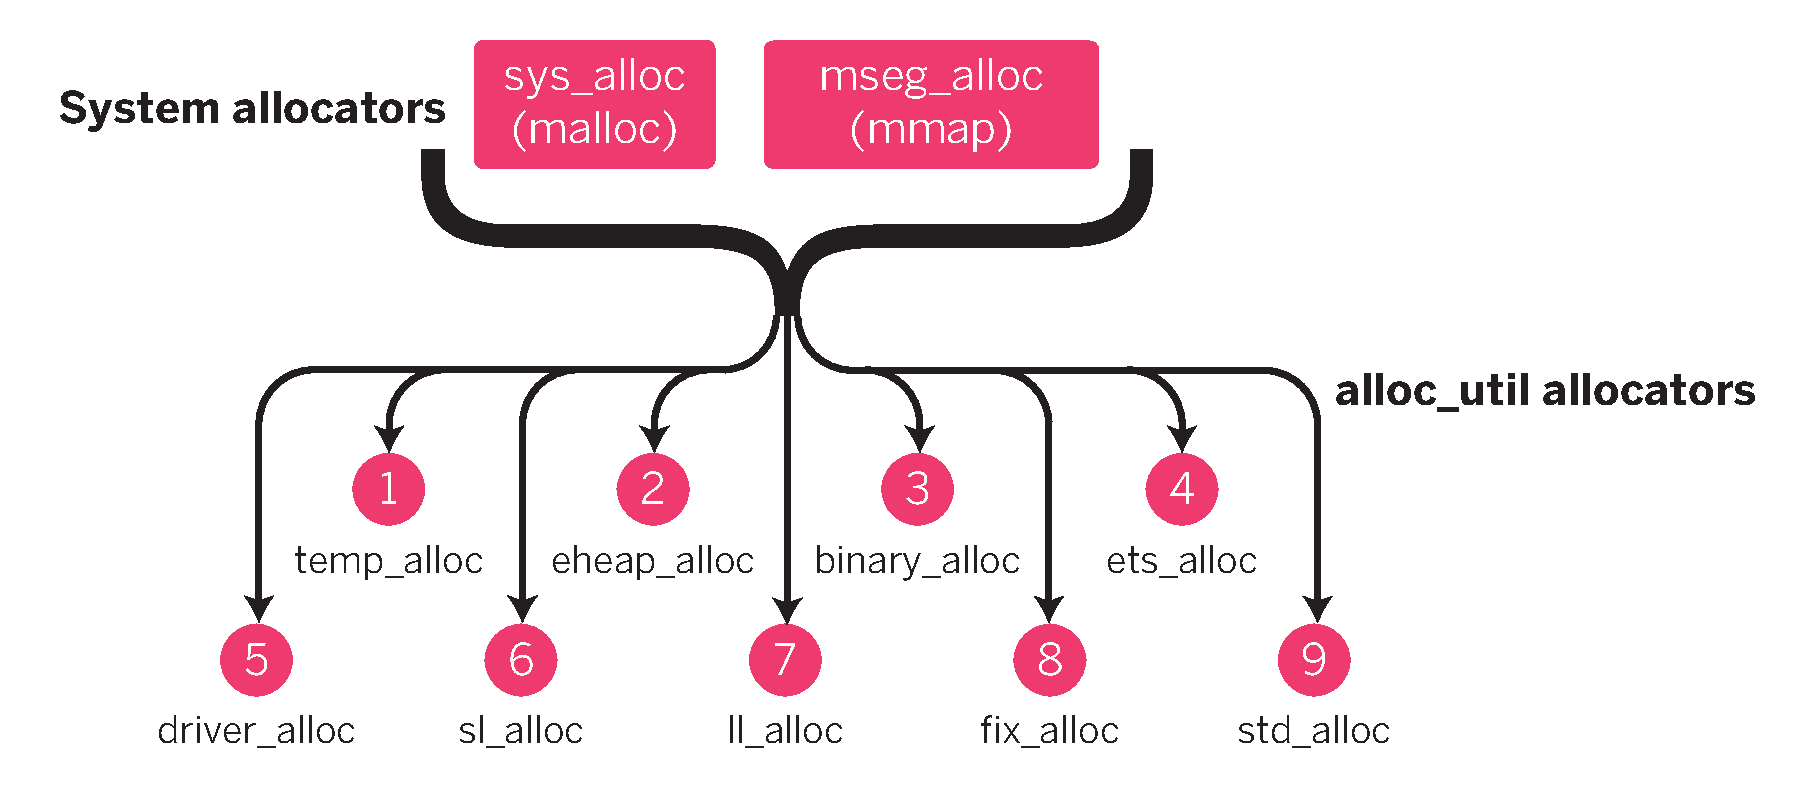
\includegraphics{memory-allocs.pdf}%
  \caption{Erlang's Memory allocators and their hierarchy. Not shown is the special \emph{super carrier}, optionally allowing to pre-allocate (and limit) all memory available to the Erlang VM since R16B03.}%
   \label{fig:allocators}
\end{figure}

\begin{enumerate*}
    \item \term{temp\_alloc}: does temporary allocations for short use cases (such as data living within a single C function call).
    \item \term{eheap\_alloc}: heap data, used for things such as the Erlang processes' heaps.
    \item \term{binary\_alloc}: the allocator used for reference counted binaries (what their 'global heap' is). Reference counted binaries stored in an ETS table remain in this allocator.
    \item \term{ets\_alloc}: ETS tables store their data in an isolated part of memory that isn't garbage collected, but allocated and deallocated as long as terms are being stored in tables.
    \item \term{driver\_alloc}: used to store driver data in particular, which doesn't keep drivers that generate Erlang terms from using other allocators. The driver data allocated here contains locks/mutexes, options, Erlang ports, etc.
    \item \term{sl\_alloc}: short-lived memory blocks will be stored there, and include items such as some of the VM's scheduling information or small buffers used for some data types' handling.
    \item \term{ll\_alloc}: long-lived allocations will be in there. Examples include Erlang code itself and the atom table, which stay there.
    \item \term{fix\_alloc}: allocator used for frequently used fixed-size blocks of memory. One example of data used there is the internal processes' C struct, used internally by the VM.
    \item \term{std\_alloc}: catch-all allocator for whatever didn't fit the previous categories. The process registry for named process is there.
\end{enumerate*}

By default, there will be one instance of each allocator per scheduler (and you should have one scheduler per core), plus one instance to be used by linked-in drivers using async threads. This ends up giving you a structure a bit like in Figure \ref{fig:allocators}, but split it in \var{N} parts at each leaf.

Each of these sub-allocators will request memory from \term{mseg\_alloc} and \term{sys\_alloc} depending on the use case, and in two possible ways. The first way is to act as a multiblock carrier (\term{mbcs}), which will fetch chunks of memory that will be used for many Erlang terms at once. For each \term{mbc}, the VM will set aside a given amount of memory (about 8MB by default in our case, which can be configured by tweaking VM options), and each term allocated will be free to go look into the many multiblock carriers to find some decent space in which to reside.

Whenever the item to be allocated is greater than the single block carrier threshold (\term{sbct})\footnote{\href{http://erlang.org/doc/man/erts\_alloc.html\#M\_sbct}{http://erlang.org/doc/man/erts\_alloc.html\#M\_sbct}}, the allocator switches this allocation into a single block carrier (\term{sbcs}). A single block carrier will request memory directly from \term{mseg\_alloc} for the first \term{mmsbc}\footnote{\href{http://erlang.org/doc/man/erts\_alloc.html\#M\_mmsbc}{http://erlang.org/doc/man/erts\_alloc.html\#M\_mmsbc}} entries, and then switch over to \term{sys\_alloc} and store the term there until it's deallocated.

So looking at something such as the binary allocator, we may end up with something similar to Figure \ref{fig:allocation-1-normal}

\begin{figure}
  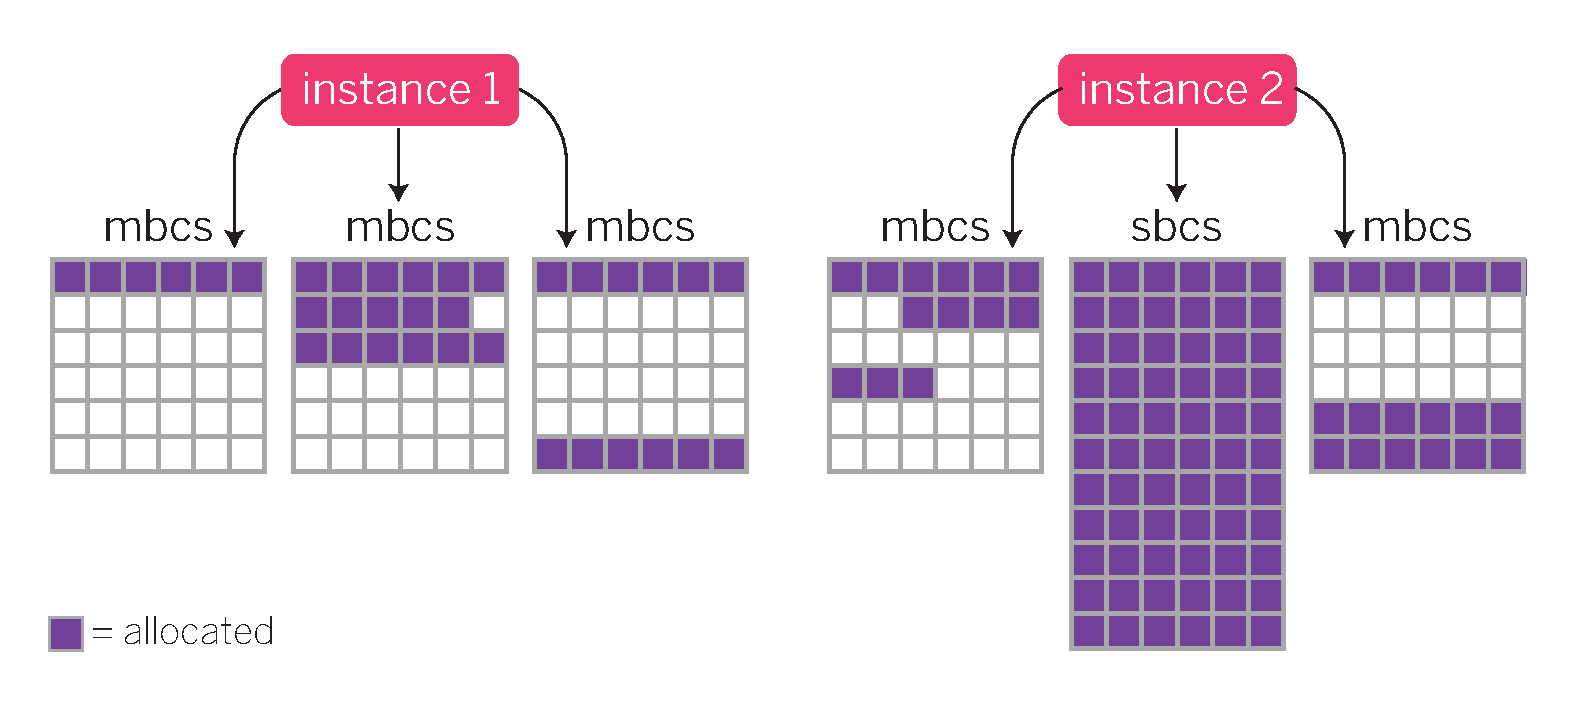
\includegraphics{allocation-1-normal.pdf}%
  \caption{Example memory allocated in a specific sub-allocator}%
   \label{fig:allocation-1-normal}
\end{figure}
\FloatBarrier

Whenever a multiblock carrier (or the first \term{mmsbc}\footnote{\href{http://erlang.org/doc/man/erts\_alloc.html\#M\_mmsbc}{http://erlang.org/doc/man/erts\_alloc.html\#M\_mmsbc}} single block carriers) can be reclaimed, \term{mseg\_alloc} will try to keep it in memory for a while so that the next allocation spike that hits your VM can use pre-allocated memory rather than needing to ask the system for more each time.

You then need to know the different memory allocation strategies of the Erlang virtual machine:

\begin{enumerate*}
    \item Best fit (\term{bf})
    \item Address order best fit (\term{aobf})
    \item Address order first fit (\term{aoff})
    \item Address order first fit carrier best fit (\term{aoffcbf})
    \item Address order first fit carrier address order best fit (\term{aoffcaobf})
    \item Good fit (\term{gf})
    \item A fit (\term{af})
\end{enumerate*}

Each of these strategies can be configured individually for each \term{alloc\_util} allocator\footnote{\href{http://erlang.org/doc/man/erts\_alloc.html\#M\_as}{http://erlang.org/doc/man/erts\_alloc.html\#M\_as}}

\begin{figure}
  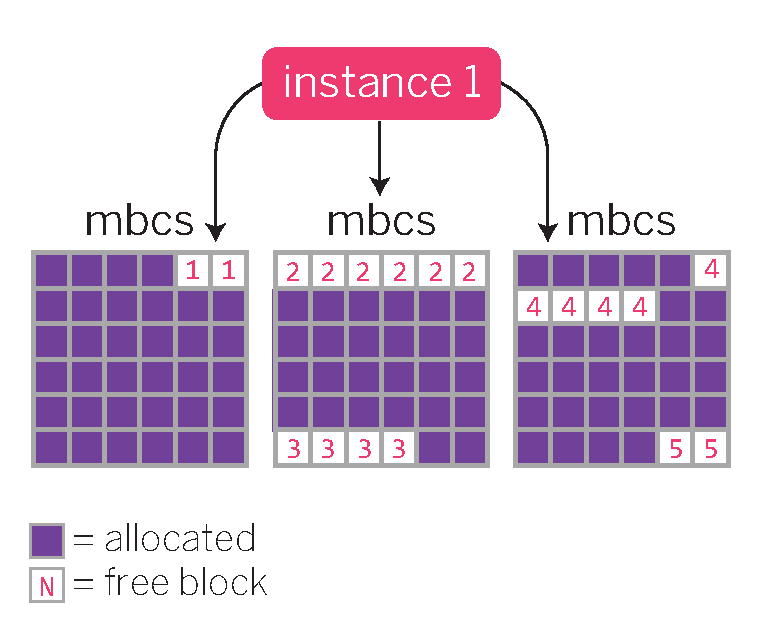
\includegraphics[max height=7cm]{allocation-strategy-1.pdf}%
  \centering%
  \caption{Example memory allocated in a specific sub-allocator}%
   \label{fig:allocation-strategy-1}
\end{figure}
\FloatBarrier

For \emph{best fit} (\term{bf}), the VM builds a balanced binary tree of all the free blocks' sizes, and will try to find the smallest one that will accommodate the piece of data and allocate it there. In Figure \ref{fig:allocation-strategy-1}, having a piece of data that requires three blocks would likely end in area 3.

\emph{Address order best fit} (\term{aobf}) will work similarly, but the tree instead is based on the addresses of the blocks. So the VM will look for the smallest block available that can accommodate the data, but if many of the same size exist, it will favor picking one that has a lower address. If I have a piece of data that requires three blocks, I'll still likely end up in area 3, but if I need two blocks, this strategy will favor the first \term{mbcs} in Figure \ref{fig:allocation-strategy-1} with area 1 (instead of area 5). This could make the VM have a tendency to favor the same carriers for many allocations.

\emph{Address order first fit} (\term{aoff}) will favor the address order for its search, and as soon as a block fits, \term{aoff} uses it. Where \term{aobf} and bf would both have picked area 3 to allocate four blocks in Figure \ref{fig:allocation-strategy-1}, this one will get area 2 as a first priority given its address is lowest. In Figure \ref{fig:allocation-strategy-2}, if we were to allocate four blocks, we'd favor block 1 to block 3 because its address is lower, whereas \term{bf} would have picked either 3 or 4, and \term{aobf} would have picked 3.

\begin{figure}
  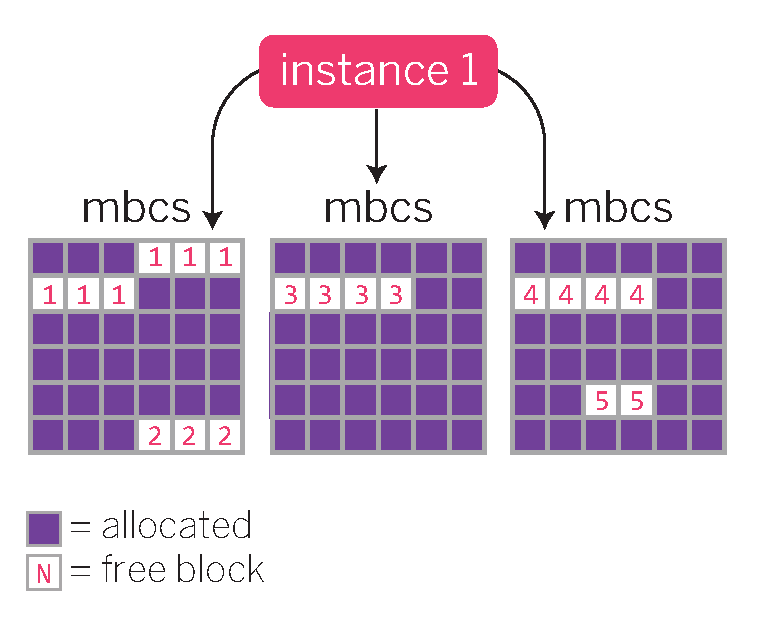
\includegraphics[max height=7cm]{allocation-strategy-2.pdf}%
  \centering%
  \caption{Example memory allocated in a specific sub-allocator}%
   \label{fig:allocation-strategy-2}
\end{figure}
\FloatBarrier

\emph{Address order first fit carrier best fit} (\term{aoffcbf}) is a strategy that will first favor a carrier that can accommodate the size and then look for the best fit within that one. So if we were to allocate two blocks in Figure \ref{fig:allocation-strategy-2}, \term{bf} and \term{aobf} would both favor block 5, \term{aoff} would pick block 1. \term{aoffcbf} would pick area 2, because the first \term{mbcs} can accommodate it fine, and area 2 fits it better than area 1.

\emph{Address order first fit carrier address order best fit} (\term{aoffcaobf}) will be similar to \term{aoffcbf}, but if multiple areas within a carrier have the same size, it will favor the one with the smallest address between the two rather than leaving it unspecified.

\emph{Good fit} (\term{gf}) is a different kind of allocator; it will try to work like best fit (\term{bf}), but will only search for a limited amount of time. If it doesn't find a perfect fit there and then, it will pick the best one encountered so far. The value is configurable through the \term{mbsd}\footnote{\href{http://www.erlang.org/doc/man/erts\_alloc.html\#M\_mbsd}{http://www.erlang.org/doc/man/erts\_alloc.html\#M\_mbsd}} VM argument.

\emph{A fit} (\term{af}), finally, is an allocator behaviour for temporary data that looks for a single existing memory block, and if the data can fit, \term{af} uses it. If the data can't fit, \term{af} allocates a new one.

Each of these strategies can be applied individually to every kind of allocator, so that the heap allocator and the binary allocator do not necessarily share the same strategy.

Finally, starting with Erlang version 17.0, each \term{alloc\_util} allocator on each scheduler has what is called a \emph{\term{mbcs} pool}. The \term{mbcs} pool is a feature used to fight against memory fragmentation on the VM. When an allocator gets to have one of its multiblock carriers become mostly empty,\footnote{The threshold is configurable through \href{http://www.erlang.org/doc/man/erts\_alloc.html\#M\_acul}{http://www.erlang.org/doc/man/erts\_alloc.html\#M\_acul}} the carrier becomes \emph{abandoned}. 

This abandoned carrier will stop being used for new allocations, until new multiblock carriers start being required. When this happens, the carrier will be fetched from the \term{mbcs} pool. This can be done across multiple \term{alloc\_util} allocators of the same type across schedulers. This allows the VM to cache mostly-empty carriers without forcing deallocation of their memory.\footnote{In cases this consumes too much memory, the feature can be disabled with the options \term{+MBacul 0}.} It also enables the migration of carriers across schedulers when they contain little data, according to their needs.

\subsubsection{The Process Level}
\label{subsec:memory-process-level}

On a smaller scale, for each Erlang process, the layout still is a bit different. It basically has this piece of memory that can be imagined as one box:

\begin{VerbatimText}
[                  ]
\end{VerbatimText}

On one end you have the heap, and on the other, you have the stack:

\begin{VerbatimText}
[heap |     | stack]
\end{VerbatimText}

In practice there's more data (you have an old heap and a new heap, for generational GC, and also a virtual binary heap, to account for the space of reference-counted binaries on a specific sub-allocator not used by the process — \term{binary\_alloc} vs. \term{eheap\_alloc}):

\begin{VerbatimText}
[heap   ||    stack]
\end{VerbatimText}

The space is allocated more and more up until either the stack or the heap can't fit in anymore. This triggers a minor GC. The minor GC moves the data that can be kept into the old heap. It then collects the rest, and may end up reallocating more space.

After a given number of minor GCs and/or reallocations, a full-sweep GC is performed, which inspects both the new and old heaps, frees up more space, and so on. When a process dies, both the stack and heap are taken out at once. reference-counted binaries are decreased, and if the counter is at 0, they vanish.

When that happens, over 80\% of the time, the only thing that happens is that the memory is marked as available in the sub-allocator and can be taken back by new processes or other ones that may need to be resized. Only after having this memory unused — and the multiblock carrier unused also — is it returned to \term{mseg\_alloc} or \term{sys\_alloc}, which may or may not keep it for a while longer.

\subsection{Fixing Memory Fragmentation with a Different Allocation Strategy}

Tweaking your VM's options for memory allocation may help.

You will likely need to have a good understanding of what your type of memory load and usage is, and be ready to do a lot of in-depth testing. The \module{recon\_alloc} module contains a few helper functions to provide guidance, and the module's documentation\footnote{\href{http://ferd.github.io/recon/recon\_alloc.html}{http://ferd.github.io/recon/recon\_alloc.html}} should be read at this point.

You will need to figure out what the average data size is, the frequency of allocation and deallocation, whether the data fits in \term{mbcs} or \term{sbcs},  and you will then need to try playing with a bunch of the options mentioned in \module{recon\_alloc}, try the different strategies, deploy them, and see if things improve or if they impact times negatively.

This is a very long process for which there is no shortcut, and if issues happen only every few months per node, you may be in for the long haul. 


\section{Exercises}

\subsection*{Review Questions}

\begin{enumerate}
	\item Name some of the common sources of leaks in Erlang programs.
	\item What are the two main types of binaries in Erlang?
	\item What could be to blame if no specific data type seems to be the source of a leak?
	\item If you find the node died with a process having a lot of memory, what could you do to find out which one it was?
	\item How could code itself cause a leak?
	\item How can you find out if garbage collections are taking too long to run?
\end{enumerate}

\subsection*{Open-ended Questions}

\begin{enumerate}
	\item  How could you verify if a leak is caused by forgetting to kill processes, or by processes using too much memory on their own?
	\item A process opens a 150MB log file in binary mode to go extract a piece of information from it, and then stores that information in an ETS table. After figuring out you have a binary memory leak, what should be done to minimize binary memory usage on the node?
	\item What could you use to find out if ETS tables are growing too fast?
	\item What steps should you go through to find out that a node is likely suffering from fragmentation? How could you disprove the idea that is could be due to a NIF or driver leaking memory?
	\item How could you find out if a process with a large mailbox (from reading \term{message\_queue\_len}) seems to be leaking data from there, or never handling new messages?
	\item A process with a large memory footprint seems to be rarely running garbage collections. What could explain this?
	\item When should you alter the allocation strategies on your nodes? Should you prefer to tweak this, or the way you wrote code?
\end{enumerate}

\subsection*{Hands-On}

\begin{enumerate}
	\item Using any system you know or have to maintain in Erlang (including toy systems), can you figure out if there are any binary memory leaks on there?
\end{enumerate}


\chapter{CPU and Scheduler Hogs}
\label{chap:cpu-hogs}

While memory leaks tend to absolutely kill your system, CPU exhaustion tends to act like a bottleneck and limits the maximal work you can get out of a node. Erlang developers will have a tendency to scale horizontally when they face such issues. It is often an easy enough job to scale out the more basic pieces of code out there. Only centralized global state (process registries, ETS tables, and so on) usually need to be modified.\footnote{Usually this takes the form of sharding or finding a state-replication scheme that's suitable, and little more. It's still a decent piece of work, but nothing compared to finding out most of your program's semantics aren't applicable to distributed systems given Erlang usually forces your hand there in the first place.} Still, if you want to optimize locally before scaling out at first, you need to be able to find your CPU and scheduler hogs.

It is generally difficult to properly analyze the CPU usage of an Erlang node to pin problems to a specific piece of code. With everything concurrent and in a virtual machine, there is no guarantee you will find out if a specific process, driver, your own Erlang code, NIFs you may have installed, or some third-party library is eating up all your processing power.

The existing approaches are often limited to profiling and reduction-counting if it's in your code, and to monitoring the scheduler's work if it might be anywhere else (but also your code).

\section{Profiling and Reduction Counts}
\label{sec:cpu-profiling}

To pin issues to specific pieces of Erlang code, as mentioned earlier, there are two main approaches. One will be to do the old standard profiling routine, likely using one of the following applications:\footnote{All of these profilers work using Erlang tracing functionality with almost no restraint. They will have an impact on the run-time performance of the application, and shouldn't be used in production.}

\begin{itemize*}
	\item \otpapp{eprof},\footnote{\href{http://www.erlang.org/doc/man/eprof.html}{http://www.erlang.org/doc/man/eprof.html}} the oldest Erlang profiler around. It will give general percentage values and will mostly report in terms of time taken.
	\item \otpapp{fprof},\footnote{\href{http://www.erlang.org/doc/man/fprof.html}{http://www.erlang.org/doc/man/fprof.html}} a more powerful replacement of eprof. It will support full concurrency and generate in-depth reports. In fact, the reports are so deep that they are usually considered opaque and hard to read. 
	\item \otpapp{eflame},\footnote{\href{https://github.com/proger/eflame}{https://github.com/proger/eflame}} the newest kid on the block. It generates flame graphs to show deep call sequences and hot-spots in usage on a given piece of code. It allows one to quickly find issues with a single look at the final result.
\end{itemize*}

It will be left to the reader to thoroughly read each of these application's documentation. The other approach will be to run \function{recon:proc\_window/3} as introduced in Subsection \ref{subsec:digging-procs}:

\begin{VerbatimEshell}
1> recon:proc_window(reductions, 3, 500).
[{<0.46.0>,51728,
  [{current_function,{queue,in,2}},
   {initial_call,{erlang,apply,2}}]},
 {<0.49.0>,5728,
  [{current_function,{dict,new,0}},
   {initial_call,{erlang,apply,2}}]},
 {<0.43.0>,650,
  [{current_function,{timer,sleep,1}},
   {initial_call,{erlang,apply,2}}]}]
\end{VerbatimEshell}

The reduction count has a direct link to function calls in Erlang, and a high count is usually the synonym of a high amount of CPU usage. 

What's interesting with this function is to try it while a system is already rather busy,\footnote{See Subsection \ref{subsec:global-cpu}} with a relatively short interval. Repeat it many times, and you should hopefully see a pattern emerge where the same processes (or the same \emph{kind} of processes) tend to always come up on top.

Using the code locations\footnote{Call \expression{recon:info(PidTerm, location)} or \expression{process\_info(Pid, current\_stacktrace)} to get this information.} and current functions being run, you should be able to identify what kind of code hogs all your schedulers.

\section{System Monitors}
\label{sec:cpu-system-monitors}

If nothing seems to stand out through either profiling or checking reduction counts, it's possible some of your work ends up being done by NIFs, garbage collections, and so on. These kinds of work may not always increment their reductions count correctly, so they won't show up with the previous methods, only through long run times.

To find about such cases, the best way around is to use \function{erlang:system\_monitor/2}, and look for \term{long\_gc} and \term{long\_schedule}. The former will show whenever garbage collection ends up doing a lot of work (it takes time!), and the latter will likely catch issues with busy processes, either through NIFs or some other means, that end up making them hard to de-schedule.\footnote{Long garbage collections count towards scheduling time. It is very possible that a lot of your long schedules will be tied to garbage collections depending on your system.}

We've seen how to set such a system monitor In Garbage Collection in \ref{subsubsec:leak-gc}, but here's a different pattern\footnote{If you're on 17.0 or newer versions, the shell functions can be made recursive far more simply by using their named form, but to have the widest compatibility possible with older versions of Erlang, I've let them as is.} I've used before to catch long-running items:

\begin{VerbatimEshell}
1> F = fun(F) ->
    receive
        {monitor, Pid, long_schedule, Info} ->
            io:format("monitor=long_schedule pid=~p info=~p~n", [Pid, Info]);
        {monitor, Pid, long_gc, Info} -> 
            io:format("monitor=long_gc pid=~p info=~p~n", [Pid, Info])
    end,
    F(F)
end.
2> Setup = fun(Delay) -> fun() -> 
     register(temp_sys_monitor, self()),
     erlang:system_monitor(self(), [{long_schedule, Delay}, {long_gc, Delay}]),
     F(F)
end end.
3> spawn_link(Setup(1000)).
<0.1293.0>
monitor=long_schedule pid=<0.54.0> info=[{timeout,1102},
                                         {in,{some_module,some_function,3}},
                                         {out,{some_module,some_function,3}}]
\end{VerbatimEshell}

Be sure to set the \term{long\_schedule} and \term{long\_gc} values to large-ish values that might be reasonable to you. In this example, they're set to 1000 milliseconds. You can either kill the monitor by calling \expression{exit(whereis(temp\_sys\_monitor), kill)} (which will in turn kill the shell because it's linked), or just disconnect from the node (which will kill the process because it's linked to the shell.)

This kind of code and monitoring can be moved to its own module where it reports to a long-term logging storage, and can be used as a canary for performance degradation or overload detection.

\subsection{Suspended Ports}
\label{subsec:port-system-monitors}

An interesting part of system monitors that didn't fit anywhere but may have to do with scheduling is regarding ports. When a process sends too many message to a port and the port's internal queue gets full, the Erlang schedulers will forcibly de-schedule the sender until space is freed. This may end up surprising a few users who didn't expect that implicit back-pressure from the VM.

This kind of event can be monitored by passing in the atom \term{busy\_port} to the system monitor. Specifically for clustered nodes, the atom \term{busy\_dist\_port} can be used to find when a local process gets de-scheduled when contacting a process on a remote node whose inter-node communication was handled by a busy port.

If you find out you're having problems with these, try replacing your sending functions where in critical paths with \function{erlang:port\_command(Port, Data, [nosuspend])} for ports, and \function{erlang:send(Pid, Msg, [nosuspend])} for messages to distributed processes. They will then tell you when the message could not be sent and you would therefore have been descheduled.


%\section{Exercises}
\section{演習}

%\subsection*{Review Questions}
\subsection*{復習問題}

\begin{enumerate}
	%\item What are the two main approaches to pin issues about CPU usages?
	\item CPU 利用率に関する問題を特定するための主なアプローチ2つとは何ですか?
	%\item Name some of the profiling tools available. What approaches are preferable for production use? Why?
	\item プロファイル用のツールの名前をいくつか挙げてください。本番環境で使用する場合、どの方法が好ましいですか? またそれはなぜですか?
	%\item Why can long scheduling monitors be useful to find CPU or scheduler over-consumption?
	\item ロングスケジュールモニターが、CPU やスケジューラの使いすぎを見つけるのに便利なのはなぜですか?

\end{enumerate}

%\subsection*{Open-ended Questions}
\subsection*{自由回答}

\begin{enumerate}
	%\item If you find that a process doing very little work with reductions ends up being scheduled for long periods of time, what can you guess about it or the code it runs?
  \item ほとんど仕事をしない(リダクションカウンタを増やさない)プロセスが長期間スケジューリングされているのを見つけた場合、そのプロセスもしくは実行しているコードについて何が考えられますか?

	%\item Can you set up a system monitor and then trigger it with regular Erlang code? Can you use it to find out for how long processes seem to be scheduled on average? You may need to manually start random processes from the shell that are more aggressive in their work than those provided by the existing system.
	\item あなたはシステムモニターを設定して、通常の Erlang コードでそれを起動できますか? プロセスが平均しておよそどれぐらいの長さスケジューリングされているかを見つけるために、システムモニターを利用できますか? 既存のシステムにすでにあるものよりもより適切にそれを行えるようなプロセスを、シェルから手動で手当たり次第に起動する必要があるかもしれません。

\end{enumerate}


%\chapter{Tracing}
\chapter{トレース}
\label{chap:tracing}

%One of the lesser known and absolutely under-used features of Erlang and the BEAM virtual machine is just about how much tracing you can do on there.
ErlangとBEAM VMの機能で、およそどれぐらいのことをトレースできるかはあまり知られておらず、また全然使われていません。

%Forget your debuggers, their use is too limited.\footnote{One common issue with debuggers that let you insert break points and step through a program is that they are incompatible with many Erlang programs: put a break point in one process and the ones around keep going. In practice, this turns debugging into a very limited activity because as soon as a process needs to interact with the one you're debugging, its calls start timing out and crashing, possibly taking down the entire node with it. Tracing, on the other hand, doesn't interfere with program execution, but still gives you all the data you need.} Tracing makes sense in Erlang at all steps of your system's life cycle, whether it's for development or for diagnosing a running production system.
使えるところが限られているので、デバッガのことは忘れてください\footnote{デバッガでブレークポイントを追加してステップ実行する時の代表的な問題は、多くのErlangプログラムとうまくやりとりができないことです。あるプロセスがブレークポイントで止まっても、その他のプロセスは動作し続けます。そのため、プロセスがデバッグ対象のプロセスとやりとりが必要なときにはすぐに、プロセス呼び出しがタイムアウトしてクラッシュし、おそらくノード全体を落としてしまいます。ですから、デバックは非常に限定的なものとなります。一方でトレースはプログラムの実行を邪魔することは無く、また必要なデータをすべて取得することができます。}。Erlangでは、トレースは開発中あるいは稼働中の本番システムの診断など、システムのライフサイクルのどこでも便利です。

%There are a few options available to trace Erlang programs:
トレースを行ういくつかのErlangプログラムがあります。


\begin{itemize}
%	\item \module{sys}\footnote{\href{http://www.erlang.org/doc/man/sys.html}{http://www.erlang.org/doc/man/sys.html}} comes standard with OTP and allows the user to set custom tracing functions, log all kinds of events, and so on. It's generally complete and fine to use for development. It suffers a bit in production because it doesn't redirect IO to remote shells, and doesn't have rate-limiting capabilities for trace messages. It is still recommended to read the documentation for the module.
	\item \module{sys}\footnote{\href{http://www.erlang.org/doc/man/sys.html}{http://www.erlang.org/doc/man/sys.html}} はOTPに標準で付属されており、利用者はトレース機能のカスタマイズや、あらゆる種類のイベントのロギングなどができます。多くの場合、開発用として完全かつ最適です。一方で、IOをリモートシェルにリダイレクトしないですし、メッセージのトレースのレート制限機能を持たないため、本番環境にはあまり向きません。このモジュールのドキュメントを読むことをお勧めします。

%	\item \otpapp{dbg}\footnote{\href{http://www.erlang.org/doc/man/dbg.html}{http://www.erlang.org/doc/man/dbg.html}} also comes standard with Erlang/OTP. Its interface is a bit clunky in terms of usability, but it's entirely good enough to do what you need. The problem with it is that you \emph{have to know what you're doing}, because \otpapp{dbg} can log absolutely everything on the node and kill one in under two seconds.
\item \otpapp{dbg}\footnote{\href{http://www.erlang.org/doc/man/dbg.html}{http://www.erlang.org/doc/man/dbg.html}}も Erlang/OTPに標準で付属しています。使い勝手の面ではインターフェースは少しイケてませんが、必要なことをやるには十分です。問題点としては、\emph{何をやっているのか知らないといけない}ということです。なぜなら \otpapp{dbg} はノードのすべてをロギングすることや、2秒もかからずにノードを落とすこともできるからです。

%	\item \emph{tracing BIFs} are available as part of the \module{erlang} module. They're mostly the raw blocks used by all the applications mentioned in this list, but their lower level of abstraction makes them rather difficult to use.
	\item \emph{トレースBIF}は \module{erlang}モジュールの一部として提供されています。このリストの全てのアプリケーションで使われているローレベルの部品ですが、抽象化が低いため、利用するのは困難です。

%\item \otpapp{redbug}\footnote{\href{https://github.com/massemanet/eper/blob/master/doc/redbug.txt}{https://github.com/massemanet/eper/blob/master/doc/redbug.txt}} is a production-safe tracing library, part of the \otpapp{eper}\footnote{\href{https://github.com/massemanet/eper}{https://github.com/massemanet/eper}} suite. It has an internal rate-limiter, and a nice usable interface. To use it, you must however be willing to add in all of \otpapp{eper}'s dependencies. The toolkit is fairly comprehensive and can be a very interesting install.
\item \otpapp{redbug}\footnote{\href{https://github.com/massemanet/eper/blob/master/doc/redbug.txt}{https://github.com/massemanet/eper/blob/master/doc/redbug.txt}} は \otpapp{eper}\footnote{\href{https://github.com/massemanet/eper}{https://github.com/massemanet/eper}} スイートの一部で、本番環境環境でも安全に使えるトレースライブラリです。内部にレート制限機能を持ち、使いやすい素敵なインターフェースを持っていますが、利用するには\otpapp{eper}が依存するもの全てを追加する必要があります。ツールキットは包括的で、またインストールは非常に面白いです。

%\item \module{recon\_trace}\footnote{\href{http://ferd.github.io/recon/recon\_trace.html}{http://ferd.github.io/recon/recon\_trace.html}} is \otpapp{recon}'s take on tracing. The objective was to allow the same levels of safety as with \otpapp{redbug}, but without the dependencies. The interface is different, and the rate-limiting options aren't entirely identical. It can also only trace function calls, and not messages.\footnote{Messages may be supported in future iterations of the library. In practice, the author hasn't found the need when using OTP, given behaviours and matching on specific arguments allows the user to get something roughly equivalent.}
\item \module{recon\_trace}\footnote{\href{http://ferd.github.io/recon/recon\_trace.html}{http://ferd.github.io/recon/recon\_trace.html}}は\otpapp{recon}によるトレースです。\otpapp{redbug}と同程度の安全性を目的としていましたが、依存関係はありません。インターフェースは異なり、またレート制限のオプションも完全に同じではありません。関数呼び出しもトレースすることができますが、メッセージのトレースはできません\footnote{メッセージのトレース機能は将来のバージョンでサポートされるかもしれません。ライブラリの著者は OTP を使っている時には必要性を感じておらず、またビヘイビアと特定の引数へのマッチングにより、ユーザはおよそ同じことを実現できます}。
\end{itemize}

この章では \module{recon\_trace} によるトレースにフォーカスしていきますが、使われている用語やコンセプトの多くは、Erlang の他のトレースツールにも活用できます。

%\section{Tracing Principles}
\section{トレースの原則}
\label{sec:tracing-princples}

%The Erlang Trace BIFs allow to trace any Erlang code at all\footnote{In cases where processes contain sensitive information, data can be forced to be kept private by calling \expression{process\_flag(sensitive, true)}}. They work in two parts: \emph{pid specifications}, and \emph{trace patterns}.
ErlangのトレースBIFは全てのErlangコードをトレースすることを可能にします\footnote{プロセスに機密情報が含まれている場合、\expression{process\_flag(sensitive, true)}を呼ぶことで、データを非公開にすることを強制できます}。BIFは\emph{pid指定}と\emph{トレースパターン}に分かれています。

%Pid specifications lets the user decide which processes to target. They can be specific pids, \expression{all} pids, \expression{existing} pids, or \expression{new} pids (those not spawned at the time of the function call).
pid指定により、ユーザはどのプロセスをターゲットにするかを決めることができます。pidは、特定のpid, \expression{全ての}pid, \expression{既存の}pid, あるいは \expression{new} pid(関数呼び出しの時点ではまだ生成されていないプロセス)で指定できます。

%The trace patterns represent functions. Functions can be specified in two parts: specifying the modules, functions, and arity, and then with Erlang match specifications\footnote{\href{http://www.erlang.org/doc/apps/erts/match\_spec.html}{http://www.erlang.org/doc/apps/erts/match\_spec.html}} to add constraints to arguments.
トレースパターンは関数の代わりになります。関数の指定は2つに分かれており、MFA(モジュール、関数、アリティ)と Erlang のマッチの仕様で引数に制約を加えています\footnote{\href{http://www.erlang.org/doc/apps/erts/match\_spec.html}{http://www.erlang.org/doc/apps/erts/match\_spec.html}}

%What defines whether a specific function call gets traced or not is the intersection of both, as seen in Figure~\ref{fig:tracing-venn}.
特定の関数呼び出しがトレースされるかどうかを定義している箇所は、~\ref{fig:tracing-venn}にあるように、両者の共通部分です。

\begin{figure}[H]
  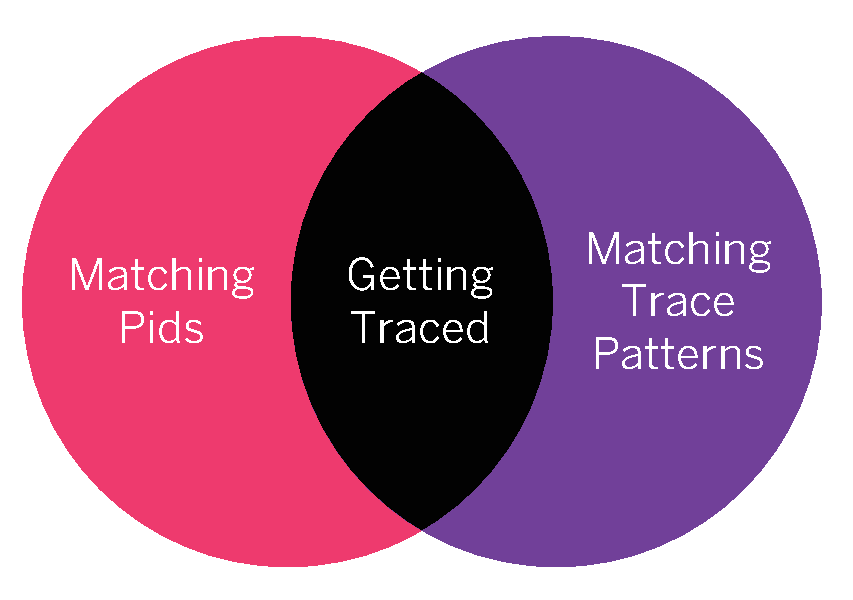
\includegraphics[max height=7cm]{tracing-venn.pdf}%
  \centering%
%  \caption{What gets traced is the result of the intersection between the matching pids and the matching trace patterns}%
  \caption{トレースされるのは、pid指定とトレースパターンの交差した箇所です}%
   \label{fig:tracing-venn}
\end{figure}

%If either the pid specification excludes a process or a trace pattern excludes a given call, no trace will be received.
pid指定がプロセスを除外、あるいはトレースパターンが指定の呼び出しを除外した場合、トレースは受信されません。

%Tools like \otpapp{dbg} (and trace BIFs) force you to work with this Venn diagram in mind. You specify sets of matching pids and sets of trace patterns independently, and whatever happens to be at the intersection of both sets gets to be displayed.
\otpapp{dbg}(およびトレースBIF)のようなツールは、このベン図を念頭に置いて作業することを前提としています。pid指定およびトレースパターンを別々に指定し、その結果が何であろうとも、両者の共通部分が表示されることになります。

%Tools like \otpapp{redbug} and \module{recon\_trace}, on the other hand, abstract this away.
一方で \otpapp{redbug}や\module{recon\_trace}のようなツールでは、これらを抽象化しています。

%\section{Tracing with Recon}
\section{Recon によるトレース}

%Recon, by default, will match all processes. This will often be good enough for a lot of debugging cases. The interesting part you'll want to play with most of the time is specification of trace patterns. Recon support a few basic ways to declare them. 
デフォルトでは Recon は全てのプロセスにマッチしますが、デバッグ時のほとんどのケースはこれで問題ありません。多くの場合、あなたがいじくりたいと思う面白い部分は、トレースするパターンの指定です。Recon ではいくつかの方法をサポートしています。

%The most basic form is \expression{\{Mod, Fun, Arity\}}, where \var{Mod} is a literal module, \var{Fun} is a function name, and \var{Arity} is the number of arguments of the function to trace. Any of these may also be replaced by wildcards (\expression{'\_'}). Recon will forbid forms that match too widely on everything (such as \expression{\{'\_','\_','\_'\}}), as they could be plain dangerous to run in production.
最も基本的な指定方法は \expression{\{Mod, Fun, Arity\}}で、\var {Mod} はモジュール名、\var{Fun}は関数名、\var{Arity} はアリティつまりトレース対象の関数の引数の数です。いずれもワイルドカードの(\expression{'\_'})で置き換えることができます。本番環境での実行は明らかに危険なため、Recon は(\expression{\{'\_','\_','\_'\}}のように)あまりにも広範囲あるいは全てにマッチするような指定は禁止しています。

%A fancier form will be to replace the arity by a function to match on lists of arguments. The function is limited to those usable by match specifications similar to what is available in ETS\footnote{\href{http://www.erlang.org/doc/man/ets.html\#fun2ms-1}{http://www.erlang.org/doc/man/ets.html\#fun2ms-1}}. Finally, multiple patterns can be put into a list to broaden the matching scope.
より賢明な方法は、アリティを引数のリストにマッチする関数で置き換えることです。その関数はETSで利用できるもの\footnote{\href{http://www.erlang.org/doc/man/ets.html\#fun2ms-1}{http://www.erlang.org/doc/man/ets.html\#fun2ms-1}}と同様に、マッチの指定で利用されるものに限定されています。また、複数のパターンをリストで指定して、マッチするパターンを増やすこともできます。

%It will also be possible to rate limit based on two manners: a static count, or a number of matches per time interval.
レート制限は静的な値によるカウントか、一定期間内にマッチした数の2つの方法で行うことができます。

%Rather than going more in details, here's a list of examples and how to trace for them.
より詳細には立ち入らず、ここではいくつかの例と、トレースの方法を見ていきます。

% \begin{VerbatimErl}
% % %% All calls from the queue module, with 10 calls printed at most:
% recon_trace:calls({queue, '_', '_'}, 10)
% 
% % %% All calls to lists:seq(A,B), with 100 calls printed at most:
% recon_trace:calls({lists, seq, 2}, 100)
% 
% % %% All calls to lists:seq(A,B), with 100 calls per second at most:
% recon_trace:calls({lists, seq, 2}, {100, 1000})
% 
% %% All calls to lists:seq(A,B,2) (all sequences increasing by two) with 100 calls
% %% at most:
% recon_trace:calls({lists, seq, fun([_,_,2]) -> ok end}, 100)
% 
% %% All calls to iolist_to_binary/1 made with a binary as an argument already
% %% (a kind of tracking for useless conversions):
% recon_trace:calls({erlang, iolist_to_binary,
%                    fun([X]) when is_binary(X) -> ok end},
%                   10)
% 
% %% Calls to the queue module only in a given process Pid, at a rate of 50 per
% %% second at most:
% recon_trace:calls({queue, '_', '_'}, {50,1000}, [{pid, Pid}])
% 
% %% Print the traces with the function arity instead of literal arguments:
% recon_trace:calls(TSpec, Max, [{args, arity}])
% 
% %% Matching the filter/2 functions of both dict and lists modules, across new
% %% processes only:
% recon_trace:calls([{dict,filter,2},{lists,filter,2}], 10, [{pid, new}])
% 
% %% Tracing the handle_call/3 functions of a given module for all new processes,
% %% and those of an existing one registered with gproc:
% recon_trace:calls({Mod,handle_call,3}, {1,100}, [{pid, [{via, gproc, Name}, new]}
% 
% %% Show the result of a given function call, the important bit being the
% %% return_trace() call or the {return_trace} match spec value.
% recon_trace:calls({Mod,Fun,fun(_) -> return_trace() end}, Max, Opts)
% recon_trace:calls({Mod,Fun,[{'_', [], [{return_trace}]}]}, Max, Opts)
% 
% \end{VerbatimErl}

\begin{VerbatimErl}
%% queue モジュールからの全ての呼び出しを、最大で10回まで出力
recon_trace:calls({queue, '_', '_'}, 10)

%% lists:seq(A,B) の全ての呼び出しを、最大で100回まで出力
recon_trace:calls({lists, seq, 2}, 100)

%% lists:seq(A,B)の全ての呼び出しを、最大で1秒あたり100回まで出力
recon_trace:calls({lists, seq, 2}, {100, 1000})

%% lists:seq(A,B,2)の全ての呼び出し(2つずつ増えていきます)を、最大で100回まで出力
recon_trace:calls({lists, seq, fun([_,_,2]) -> ok end}, 100)

%% 引数としてバイナリを指定して呼び出されたiolist_to_binary/1への全ての呼び出し
%% (意味のない変換をトラッキングしている一例)
recon_trace:calls({erlang, iolist_to_binary,
                   fun([X]) when is_binary(X) -> ok end},
                  10)

%% 指定の Pid から queue モジュールの呼び出しを、最大で1秒あたり50回まで
recon_trace:calls({queue, '_', '_'}, {50,1000}, [{pid, Pid}])

%% リテラル引数のかわりに、関数のアリティでトレースを出力
recon_trace:calls(TSpec, Max, [{args, arity}])

%% dict と lists モジュールの filter/2 関数にマッチして、かつ new プロセスからの呼び出しのみ
recon_trace:calls([{dict,filter,2},{lists,filter,2}], 10, [{pid, new}])

%% 指定モジュールの handle_call/3 関数の、new プロセスおよび
%% gproc で登録済の既存プロセスからの呼び出しをトレース
recon_trace:calls({Mod,handle_call,3}, {1,100}, [{pid, [{via, gproc, Name}, new]}

%% 指定の関数呼び出しの結果を表示します。重要なポイントは、
%% return_trace()の呼び出しもしくは {return_trace} へのマッチです
recon_trace:calls({Mod,Fun,fun(_) -> return_trace() end}, Max, Opts)
recon_trace:calls({Mod,Fun,[{'_', [], [{return_trace}]}]}, Max, Opts)

\end{VerbatimErl}

%Each call made will override the previous one, and all calls can be cancelled with \function{recon\_trace:clear/0}.
各々の呼び出しはそれ以前の呼び出しを上書きし、また全ての呼び出しは \function{recon\_trace:clear/0} でキャンセルすることができます。

%There's a few more combination possible, with more options:
組み合わせることが可能なオプションはもう少しあります。


\begin{description}
  \item[\expression{\{pid, PidSpec\}}] \hfill
%    Which processes to trace. Valid options is any of \term{all}, \term{new}, \term{existing}, or a process descriptor (\expression{\{A,B,C\}}, \expression{"<A.B.C>"}, an atom representing a name, \expression{\{global, Name\}}, \expression{\{via, Registrar, Name\}}, or a pid). It's also possible to specify more than one by putting them in a list.
	
	トレースするプロセスの指定です。有効なオプションは \term{all}, \term{new}, \term{existing}, あるいはプロセスディスクリプタ(\expression{\{A,B,C\}}, \expression{"<A.B.C>"}, 名前をあらわすアトム、\expression{\{global, Name\}}, \expression{\{via, Registrar, Name\}}, あるいは pid)のどれかです。リストにすることで、複数指定することも可能です。

  \item[\expression{\{timestamp, formatter | trace\}}] \hfill

%    By default, the formatter process adds timestamps to messages received. If accurate timestamps are required, it's possible to force the usage of timestamps within trace messages by adding the option \expression{\{timestamp, trace\}}.
デフォルトでは formatter プロセスは受信したメッセージにタイムスタンプを追加します。正確なタイムスタンプが必要な場合、\expression{\{timestamp, trace\}} オプションを追加することで、トレースするメッセージの中のタイムスタンプを使うことを強制できます。

  \item[\expression{\{args, arity | args\}}] \hfill

%    Whether to print the arity in function calls or their (by default) literal representation.
    関数呼び出しでアリティを表示するか、(デフォルトの)リテラル表現を出力するか

  \item[\expression{\{scope, global | local\}}] \hfill

%		By default, only 'global' (fully qualified function calls) are traced, not calls made internally. To force tracing of local calls, pass in \expression{\{scope, local\}}. This is useful whenever you want to track the changes of code in a process that isn't called with \expression{Module:Fun(Args)}, but just \expression{Fun(Args)}.
    デフォルトでは 'global'(明示的な関数呼び出し)だけがトレースされ、内部的な呼び出しはトレースされません。ローカルの呼び出しのトレースを強制するには、\expression{\{scope, local\}} を渡します。これは、\expression{Module:Fun(Args)}ではなく\expression{Fun(Args)}だけで呼び出される、プロセス内のコード変更をトラッキングしたいときに便利です。

\end{description}

%With these options, the multiple ways to pattern match on specific calls for specific functions and whatnot, a lot of development and production issues can more quickly be diagnosed. If the idea ever comes to say "hm, maybe I should add more logging there to see what could cause that funny behaviour", tracing can usually be a very fast shortcut to get the data you need without deploying any code or altering its readability.
特定の関数の特定の呼び出しやらをパターンマッチするこれらのオプションにより、開発環境・本番環境の多くの問題点をより早く診断できます。

「うーん、このおかしな挙動を引き起こしているのは何なのか、たぶんもっと多くのログを吐けばわかるかもしれない」という発想になったときには、通常はトレースすることが、デプロイや(ログを)読みやすいように変更しなくても必要なデータを入手することができる近道となります。

%\section{Example Sessions}
\section{実行例}

%First let's trace the queue:new functions in any process:
最初に、どこかのプロセスの queue:new 関数をトレースしてみましょう

\begin{VerbatimEshell}
1> recon_trace:calls({queue, new, '_'}, 1).
1
13:14:34.086078 <0.44.0> queue:new()
Recon tracer rate limit tripped.
\end{VerbatimEshell}

%The limit was set to 1 trace message at most, and recon let us know when that limit was reached.
最大1メッセージに制限されているため、recon が制限に達したことを知らせてくれます。

%Let's instead look for all the \function{queue:in/2} calls, to see what it is we're inserting in queues:
全ての\function{queue:in/2}呼び出しを見て、queue に挿入される内容をみてみましょう。

\begin{VerbatimEshell}
2> recon_trace:calls({queue, in, 2}, 1).
1
13:14:55.365157 <0.44.0> queue:in(a, {[],[]})
Recon tracer rate limit tripped.
\end{VerbatimEshell}

%In order to see the content we want, we should change the trace patterns to use a fun that matches on all arguments in a list (\term{\_}) and returns \expression{return\_trace()}. This last part will generate a second trace for each call that includes the return value:
希望する内容を見るために、トレースパターンをリスト中の全引数にマッチする fun(\term{\_})を使うように変更して、\expression{return\_trace()}を返します。この最後の部分は、リターン値を含む各々の呼び出しのトレースそのものを生成します。

\begin{VerbatimEshell}
3> recon_trace:calls({queue, in, fun(_) -> return_trace() end}, 3).
1

13:15:27.655132 <0.44.0> queue:in(a, {[],[]})

13:15:27.655467 <0.44.0> queue:in/2 --> {[a],[]}

13:15:27.757921 <0.44.0> queue:in(a, {[],[]})
Recon tracer rate limit tripped.
\end{VerbatimEshell}

%Matching on argument lists can be done in a more complex manner:
引数リストのマッチは、より複雑な方法で行うことができます。


\begin{VerbatimEshell}
4> recon_trace:calls(
4>   {queue, '_',
4>    fun([A,_]) when is_list(A); is_integer(A) andalso A > 1 ->
4>        return_trace()
4>    end},
4>   {10,100}
4> ).
32

13:24:21.324309 <0.38.0> queue:in(3, {[],[]})

13:24:21.371473 <0.38.0> queue:in/2 --> {[3],[]}

13:25:14.694865 <0.53.0> queue:split(4, {[10,9,8,7],[1,2,3,4,5,6]})

13:25:14.695194 <0.53.0> queue:split/2 --> {{[4,3,2],[1]},{[10,9,8,7],[5,6]}}

5> recon_trace:clear().
ok
\end{VerbatimEshell}

%Note that in the pattern above, no specific function (\expression{'\_'}) was matched against. Instead, the fun used restricted functions to those having two arguments, the first of which is either a list or an integer greater than 1.
上記のパターンでは、特定の関数(\expression{'\_'})にはマッチしていないことに注意してください。fun は2つの引数を持つ関数に限定され、また最初の引数はリストもしくは1よりも大きい数値です。

%Be aware that extremely broad patterns with lax rate-limitting (or very high absolute limits) may impact your node's stability in ways \module{recon\_trace} cannot easily help you with. Similarly, tracing extremely large amounts of function calls (all of them, or all of \module{io} for example) can be risky if more trace messages are generated than any process on the node could ever handle, despite the precautions taken by the library.
レート制限を緩めて非常に広範囲にマッチするパターン(あるいは制限を非常に高い数値にする)にした場合、ノードの安定性に影響を与える可能性があり、また\module{recon\_trace}はそれに対して何も支援できなくなるかもしれないということに注意してください。同様に、非常に大量の関数呼び出し(関数や\module{io}の全ての呼び出しなど)をトレースした場合、ライブラリで注意していはいますが、そのノードが処理できるプロセスよりも多くのトレースメッセージが生成されるリスクがあります。

%In doubt, start with the most restrictive tracing possible, with low limits, and progressively increase your scope.
よくわからない場合、最も制限した量でトレースを開始し、少しずつ増やしていってください。

%\section{Exercises}
\section{演習}

%\subsection*{Review Questions}
\subsection*{復習問題}

\begin{enumerate}
	%\item Why is debugger use generally limited on Erlang?
	\item Erlangでは通常なぜデバッガの使用が制限されていますか?
	%\item What are the options you can use to trace OTP processes?
	\item OTPプロセスをトレースする時に使用できるオプションは?
	%\item What determines whether a given set of functions or processes get traced?
	\item 指定の関数やプロセスがトレースされるかどうかを決めるのは何?
	%\item How can you stop tracing with \module{recon\_trace}? With other tools?
	\item \module{recon\_trace}あるいはその他のツールで、トレースを止める方法は?
	%\item How can you trace non-exported function calls?
	\item エクスポートされていない関数の呼び出しをトレースする方法は?
\end{enumerate}

%\subsection*{Open-ended Questions}
\subsection*{自由回答}

\begin{enumerate}
	%\item When would you want to move time stamping of traces to the VM's trace mechanisms directly? What would be a possible downside of doing this?	
	\item トレースにタイムスタンプを記録する時に、VMのトレース機能を直接利用するようにしたくなるのはどういう時ですか? これによる欠点は何ですか?
	%\item Imagine that traffic sent out of a node does so over SSL, over a multi-tenant system. However, due to wanting to validate data sent (following a customer complain), you need to be able to inspect what was seen clear text. Can you think up a plan to be able to snoop in the data sent to their end through the \module{ssl} socket, without snooping on the data sent to any other customer?
	\item ノードから送信されるトラフィックがSSL経由の、マルチテナントシステムを想像してみてください。ただし、(顧客からのクレームに対応するため)送信されるデータをバリデートしたいので、平文で中身を参照できる必要があります。\module{ssl}ソケット経由で送信されたデータを覗くための方法を考えられますか? しかも、その他の顧客宛のデータは覗かずにです。
\end{enumerate}

%\subsection*{Hands-On}
\subsection*{ハンズオン}

%Using the code at \href{https://github.com/ferd/recon\_demo}{https://github.com/ferd/recon\_demo} (these may require a decent understanding of the code there):
\href{https://github.com/ferd/recon\_demo}{https://github.com/ferd/recon\_demo}にあるコードを利用してください(コードの中身をきちんと理解している必要があるかもしれません)

\begin{enumerate}
	%\item Can chatty processes (\module{council\_member}) message themselves? (\emph{hint: can this work with registered names? Do you need to check the chattiest process and see if it messages itself?})
	\item メッセージを吐きまくるプロセス(\module{council\_member})は自身にメッセージを送ることができますか? (\emph{ヒント:これは登録された名前(register\_name)で動作しますか? その吐きまくるプロセスを確認、また、自身にメッセージを送ったかを知る必要はありますか?})
	%\item Can you estimate the overall frequency at which messages are sent globally?
	\item 全体で送られるメッセージの頻度を見積もることはできますか?
	%\item Can you crash a node using any of the tracing tools? (\emph{hint: dbg makes it easier due to its greater flexibility})
	\item いずれかのトレースツールを使って、ノードをクラッシュさせることはできますか?(\emph{ヒント:非常に柔軟性が高いので、dbg を使うと簡単です})
\end{enumerate}



%%%
%%% Tuning the VM: not a chapter yet.
%%%


%% locks!

%% you usually want the lmbcs to be at least a 5 times (if not more) bigger than the perc95

%% the binaries will still count as binary data if you move it to ets. It is only the pointer to the binary that moves from the heap to ets. (for binaries > 64 bytes)

%% Cache hits

%% Kernel Polling

%%
\bookmarksetup{startatroot} % Split conclusion from previous Part
\addtocontents{toc}{\bigskip} % Add space in ToC
%\chapter*{Conclusion}
\chapter*{おわりに}
 \markboth{\MakeUppercase{Conclusion}}{}
\addcontentsline{toc}{chapter}{Conclusion}


%Maintaining and debugging software never ends. New bugs and confusing behaviours will keep popping up around the place all the time. There would probably be enough stuff out there to fill out dozens of manuals like this one, even when dealing with the cleanest of all systems.
ソフトウェアの運用とデバッグは決して終わることはありません。新しいバグやややこしい動作がつねにあちこちに出現しつづけるでしょう。
いかに整ったシステムを扱う場合でも、おそらく本書のようなマニュアルを何十も書けるくらいのことがあるでしょう。

%I hope that after reading this text, the next time stuff goes bad, it won't go \emph{too} bad. Still, there are probably going to be plenty of opportunities to debug production systems. Even the most solid bridges need to be repainted all the time in order avoid corrosion to the point of their collapse.
本書を読んだことで、次に何か悪いことが起きたとしても、\emph{それほど}悪いことにはならないことを願っています。
それでも、本番システムをデバッグする機会がおそらく山ほどあることでしょう。
いかなる堅牢な橋でも腐食しないように常にペンキを塗り替えるわけです。

%Best of luck to you.
みなさんのシステム運用がうまく行くことを願っています。



\end{document}
